% Compile: latexmk -pdf -interaction=nonstopmode -halt-on-error main.tex
\documentclass{article}
\usepackage[a4paper,left=1in,right=1in,top=0.9in,bottom=1in]{geometry}
\usepackage[utf8]{vntex}
\usepackage{graphicx,float,amsmath,amssymb}
\usepackage[table,dvipsnames]{xcolor}
\usepackage{array,tabularx,longtable,booktabs,multirow}
\usepackage{caption,enumitem}
\usepackage{fancyhdr,lastpage,parskip,indentfirst}
\PassOptionsToPackage{obeyspaces}{url}
\usepackage{pdflscape,listings,xurl}
\usepackage{hyperref}
\numberwithin{figure}{section}
\numberwithin{table}{section}
\numberwithin{equation}{section}
\captionsetup{font=small,labelfont=bf}
\setlist{nosep}
\setlength{\headheight}{30pt}\addtolength{\topmargin}{-4pt}
\setlength{\parindent}{2em}
\renewcommand{\baselinestretch}{1.3}
\emergencystretch=2em
\newcolumntype{Y}{>{\raggedright\arraybackslash}X}
\newcommand{\code}[1]{{\urlstyle{same}\nolinkurl{#1}}}
\newcommand{\sourcepath}[1]{\par{\footnotesize\textit{Bằng chứng:} \code{#1}}}
\lstset{basicstyle=\ttfamily\footnotesize,breaklines=true,columns=fullflexible,
  keepspaces=true,frame=single,showstringspaces=false,keywordstyle=\color{blue!60!black},
  aboveskip=0.7em,belowskip=0.7em}
\hypersetup{colorlinks=true,linkcolor=black,urlcolor=blue!65!black,citecolor=green!45!black,
  pdftitle={OList - Kho du lieu va He ho tro quyet dinh},pdfpagemode=UseNone}
\pagestyle{fancy}\fancyhf{}
\fancyhead[L]{\begin{tabular}{rl}
\begin{picture}(25,15)(0,0)\put(0,-8){
\includegraphics[width=8mm,height=8mm]{assets/hcmut.png}}\end{picture}&
\begin{tabular}{l}\textbf{\ttfamily Trường Đại học Bách Khoa}\\
\textbf{\ttfamily Khoa Khoa học và Kỹ thuật Máy tính}\end{tabular}\end{tabular}}
\fancyfoot[L]{\scriptsize\ttfamily CO4031 -- Kho dữ liệu và Hệ hỗ trợ Quyết định. HK261}
\fancyfoot[R]{\scriptsize\ttfamily Trang \thepage/\pageref{LastPage}}
\renewcommand{\headrulewidth}{0.1pt}\renewcommand{\footrulewidth}{0.1pt}
\AtBeginDocument{\renewcommand*\contentsname{Mục lục}
\renewcommand*\listfigurename{Danh sách hình ảnh}
\renewcommand*\listtablename{Danh sách bảng}
\renewcommand*\refname{Tài liệu tham khảo}}
\begin{document}
\begin{titlepage}
\begin{center}
ĐẠI HỌC QUỐC GIA TP. HỒ CHÍ MINH\\
TRƯỜNG ĐẠI HỌC BÁCH KHOA\\
KHOA KHOA HỌC VÀ KỸ THUẬT MÁY TÍNH
\vspace{0.6cm}


\includegraphics[width=4.5cm]{assets/hcmut.png}

\vspace{0.5cm}
{\LARGE\textbf{Báo cáo Bài tập lớn}}\\[0.5cm]
{\Large\textbf{Kho dữ liệu và Hệ hỗ trợ Quyết định}}\\[0.3cm]
{\Large\textbf{CO4031 -- Học kỳ 261}}

\vspace{0.4cm}\rule{14cm}{0.1pt}\\[0.4cm]
{\LARGE\textbf{Phân tích doanh số và dự báo nhập hàng}}\\[0.2cm]
\rule{14cm}{0.1pt}
\vspace{0.5cm}

\begin{table}[h]
\centering
\begin{tabular}{l l l l}
    \textbf{GVHD}:      & Đỗ Thanh Thái &          &     \\  [3pt]
    \textbf{Nhóm}:      & 16             &          &     \\  [3pt]
    \textbf{Sinh viên}: & Nguyễn Quỳnh Như & 2312535  &  L01 \\
                        & Lê Hồng Ngọc & 2312303  &  L01 \\
                        & Dương Khả Vân & 2313866  &  L01 \\
\end{tabular}
\end{table}

\vspace{3.5cm}
% \vfill
{\small TP. Hồ Chí Minh, tháng 11 năm 2026}
\end{center}
\end{titlepage}
\setcounter{page}{2}
\tableofcontents
\clearpage\phantomsection\addcontentsline{toc}{section}{\listfigurename}\listoffigures
\clearpage\phantomsection\addcontentsline{toc}{section}{\listtablename}\listoftables
\clearpage
\section*{Thông tin báo cáo và từ viết tắt}
\addcontentsline{toc}{section}{Thông tin báo cáo và từ viết tắt}
Báo cáo trình bày bài tập lớn CO4031 học kỳ 261 về việc xây dựng kho dữ liệu đa chiều cho bộ dữ liệu thương mại điện tử OList, phân tích OLAP qua giao diện web và một hệ hỗ trợ quyết định (DSS) dự báo nhu cầu để đề xuất lượng nhập hàng. Số liệu được đo trên kho PostgreSQL sau khi chạy đầy đủ quy trình nạp dữ liệu và đối chiếu lại với các tệp CSV.

\begin{table}[H]\centering\small
\begin{tabularx}{\linewidth}{lY}
\toprule Từ viết tắt & Diễn giải\\\midrule
DW & Data Warehouse -- kho dữ liệu\\
ETL / ELT & Trích xuất, biến đổi, nạp / trích xuất, nạp, biến đổi\\
OLAP / ROLAP & Phân tích đa chiều / triển khai phân tích trên CSDL quan hệ\\
DSS & Decision Support System -- hệ hỗ trợ quyết định\\
PK / FK & Khóa chính / khóa ngoại\\
KPI / AOV & Chỉ số đánh giá / giá trị thanh toán trung bình mỗi đơn có dữ liệu\\
MoM / QoQ / YoY & So với tháng, quý, năm trước (cùng kỳ)\\
WAPE & Weighted Absolute Percentage Error -- tổng sai số tuyệt đối chia tổng giá trị thực\\
MASE & Mean Absolute Scaled Error -- sai số tuyệt đối chia sai số của dự báo ``tháng trước''\\
\bottomrule\end{tabularx}
\caption{Từ viết tắt}
\end{table}
\clearpage
\section*{Thành viên và phân công}
\phantomsection\addcontentsline{toc}{section}{Thành viên và phân công}
Dự án gồm bốn giai đoạn là phân tích câu hỏi nghiệp vụ, ETL, OLAP và DSS. Nhiệm vụ của từng thành viên như sau.

\begin{table}[H]\centering\small
\begin{tabularx}{\linewidth}{l l l Y r}
\toprule Họ và tên & MSSV & Lớp & Nhiệm vụ & Mức đóng góp\\\midrule
Nguyễn Quỳnh Như & 2312535 & L01 & Phân tích câu hỏi nghiệp vụ; OLAP màn Khách hàng; viết báo cáo phần ETL và OLAP & 100\%\\
Lê Hồng Ngọc & 2312303 & L01 & Phân tích câu hỏi nghiệp vụ; ETL; OLAP màn Thời gian; DSS; viết báo cáo phần DSS & 100\%\\
Dương Khả Vân & 2313866 & L01 & Phân tích câu hỏi nghiệp vụ; ETL; OLAP màn Khu vực và Người bán; DSS & 100\%\\
\bottomrule\end{tabularx}
\caption{Thành viên nhóm 16}
\end{table}

\clearpage\section{Bài toán, phạm vi và yêu cầu}
\subsection{Bối cảnh và mục tiêu}
Dự án dùng bộ dữ liệu giao dịch thương mại điện tử OList để tổ chức một kho dữ liệu phục vụ quản lý kinh doanh. Hệ thống gồm ba lớp: (1) kho dữ liệu đa chiều nạp từ CSV qua staging; (2) phân tích OLAP qua API Flask và giao diện React; (3) một DSS dự báo nhu cầu tháng tới và đề xuất lượng nhập hàng.

Các nhu cầu nghiệp vụ gồm xác định danh mục, thị trường và người bán đóng góp lớn, theo dõi doanh số theo thời gian, đánh giá khách mua lại và hỗ trợ quyết định nhập hàng. Phần đánh giá ban đầu về phân khúc khách hàng (RFM, K-Means) đã được thử trên dữ liệu thật nhưng cho tín hiệu yếu; lý do chọn hướng dự báo nhu cầu được trình bày ở chương~\ref{sec:dss}.

\subsection{Đối chiếu yêu cầu và kết quả}
\begingroup\small\renewcommand{\arraystretch}{1.18}
\begin{longtable}{>{\raggedright\arraybackslash}p{0.22\linewidth}>{\raggedright\arraybackslash}p{0.40\linewidth}>{\raggedright\arraybackslash}p{0.30\linewidth}}
\caption{Đối chiếu yêu cầu và kết quả}\label{tab:requirements}\\
\toprule Yêu cầu & Kết quả & Chương\\\midrule\endfirsthead
\toprule Yêu cầu & Kết quả & Chương\\\midrule\endhead
\bottomrule\endfoot
Nghiệp vụ & Chín câu hỏi phân tích (bảng~\ref{tab:bq}) và một câu hỏi quyết định & 1\\
DW đa chiều, ETL & Hai fact, bốn dimension; raw $\rightarrow$ staging $\rightarrow$ DW; nghiệm thu F1--F7 & 3, 4\\
Backend và OLAP & Flask; ba nhóm API Thời gian, Khu vực/Người bán, Khách hàng & 5\\
Frontend & Sáu màn: Tổng quan, Thời gian, Khu vực, Người bán, Khách hàng, Quyết định & 5, 6\\
Thành phần DSS & Dự báo nhu cầu theo tháng, lượng nhập đề xuất, đường đánh đổi thiếu/dư hàng & 6\\
Đánh giá kết quả & Đối soát tổng tiền, KPI, backtest DSS & 7\\
\bottomrule
\end{longtable}\endgroup

\subsection{Câu hỏi phân tích}
\begin{table}[H]\centering\small\renewcommand{\arraystretch}{1.15}
\begin{tabularx}{\linewidth}{lYY}
\toprule Mã & Câu hỏi nghiệp vụ & Thước đo và nơi xử lý\\\midrule
BQ1 & Tiền hàng theo tháng, quý, năm thay đổi thế nào? & Doanh thu hàng, MoM/QoQ/YoY; màn Thời gian.\\
BQ2 & Danh mục nào đóng góp tiền hàng lớn nhất? & Doanh thu theo danh mục; màn Khu vực.\\
BQ3 & Người bán nào tạo nhiều tiền hàng? & Doanh thu theo seller; màn Người bán.\\
BQ4 & Bang, thành phố nào mua nhiều? & Doanh thu và số đơn theo địa lý khách; màn Khu vực.\\
BQ5 & Cước vận chuyển chiếm tỷ lệ bao nhiêu so với giá? & Cước/Doanh thu hàng; Tổng quan và Khu vực.\\
BQ6 & Giá trị thanh toán trung bình mỗi đơn là bao nhiêu? & AOV trên đơn có dữ liệu thanh toán.\\
BQ7 & Bao nhiêu khách mua lại? & Số đơn delivered theo khách duy nhất; màn Khách hàng.\\
BQ8 & Khách mua và chi tiêu thế nào theo bang, năm, trạng thái đơn? & Drill-down, dice, ma trận bang $\times$ năm.\\
BQ9 & Các trạng thái đơn phân bố ra sao? & Đếm mọi trạng thái; tiền chỉ tính đơn delivered.\\
BQ10 & Tháng tới bán được bao nhiêu và nên nhập bao nhiêu? & DSS, màn Quyết định.\\
\bottomrule\end{tabularx}
\caption{Câu hỏi phân tích}\label{tab:bq}
\end{table}

\subsection{Phạm vi dữ liệu và khái niệm doanh số}
Kho lưu mọi trạng thái đơn. Các KPI bán hàng và khách hàng mặc định lọc \code{order_status = 'delivered'}; thống kê trạng thái dùng toàn bộ đơn. Tiền hàng (\code{price}), cước (\code{freight_value}) và thanh toán (\code{total_payment_value}) là ba thước đo riêng. ``Doanh thu hàng'' là tổng \code{price}, không đồng nhất với tiền thanh toán hay lợi nhuận; dữ liệu không có giá vốn.

Loại thanh toán (\code{payment_type}), số kỳ trả góp, đánh giá (review) và geolocation chỉ có ở CSV, không được đưa vào staging có kiểu hay DW. Vì vậy câu hỏi về phương thức thanh toán và các phân tích dựa trên review hay thời gian giao hàng nằm ngoài phạm vi hệ thống.

\clearpage\section{Nguồn dữ liệu và kiến trúc hệ thống}
\subsection{Dữ liệu nguồn}
Nguồn là Brazilian E-Commerce Public Dataset by Olist (Kaggle) \cite{olist}, gồm chín tệp CSV đi kèm dự án. Số bản ghi được đếm bằng bộ phân tích CSV chuẩn (không đếm dòng văn bản vì trường nhận xét có thể chứa xuống dòng).

\begin{table}[H]\centering\small
\begin{tabularx}{\linewidth}{Yrr}
\toprule Tệp CSV (rút gọn tên) & Số bản ghi & Được nạp\\\midrule
customers & 99.441 & Có \\
orders & 99.441 & Có \\
order\_items & 112.650 & Có \\
order\_payments & 103.886 & Có \\
products & 32.951 & Có \\
sellers & 3.095 & Có \\
product\_category\_name\_translation & 71 & Có \\
geolocation & 1.000.163 & Không \\
order\_reviews & 99.224 & Không \\
\bottomrule\end{tabularx}
\caption{Kiểm kê dữ liệu nguồn}
\end{table}

Bảy tệp được nạp (khai báo trong \code{RAW_TABLE_FILES}). Khách hàng có hai mã, trong đó \code{customer_id} nối với đơn, còn \code{customer_unique_id} nhận diện một người mua qua nhiều đơn. Bảng sản phẩm có thể thiếu danh mục; bản dịch được nối trái để không loại sản phẩm. Mỗi dòng order item là một mục trong đơn; \code{order_item_id} là số thứ tự trong đơn, không phải số lượng.

\subsection{Kiến trúc và luồng xử lý}
\begin{figure}[H]\centering
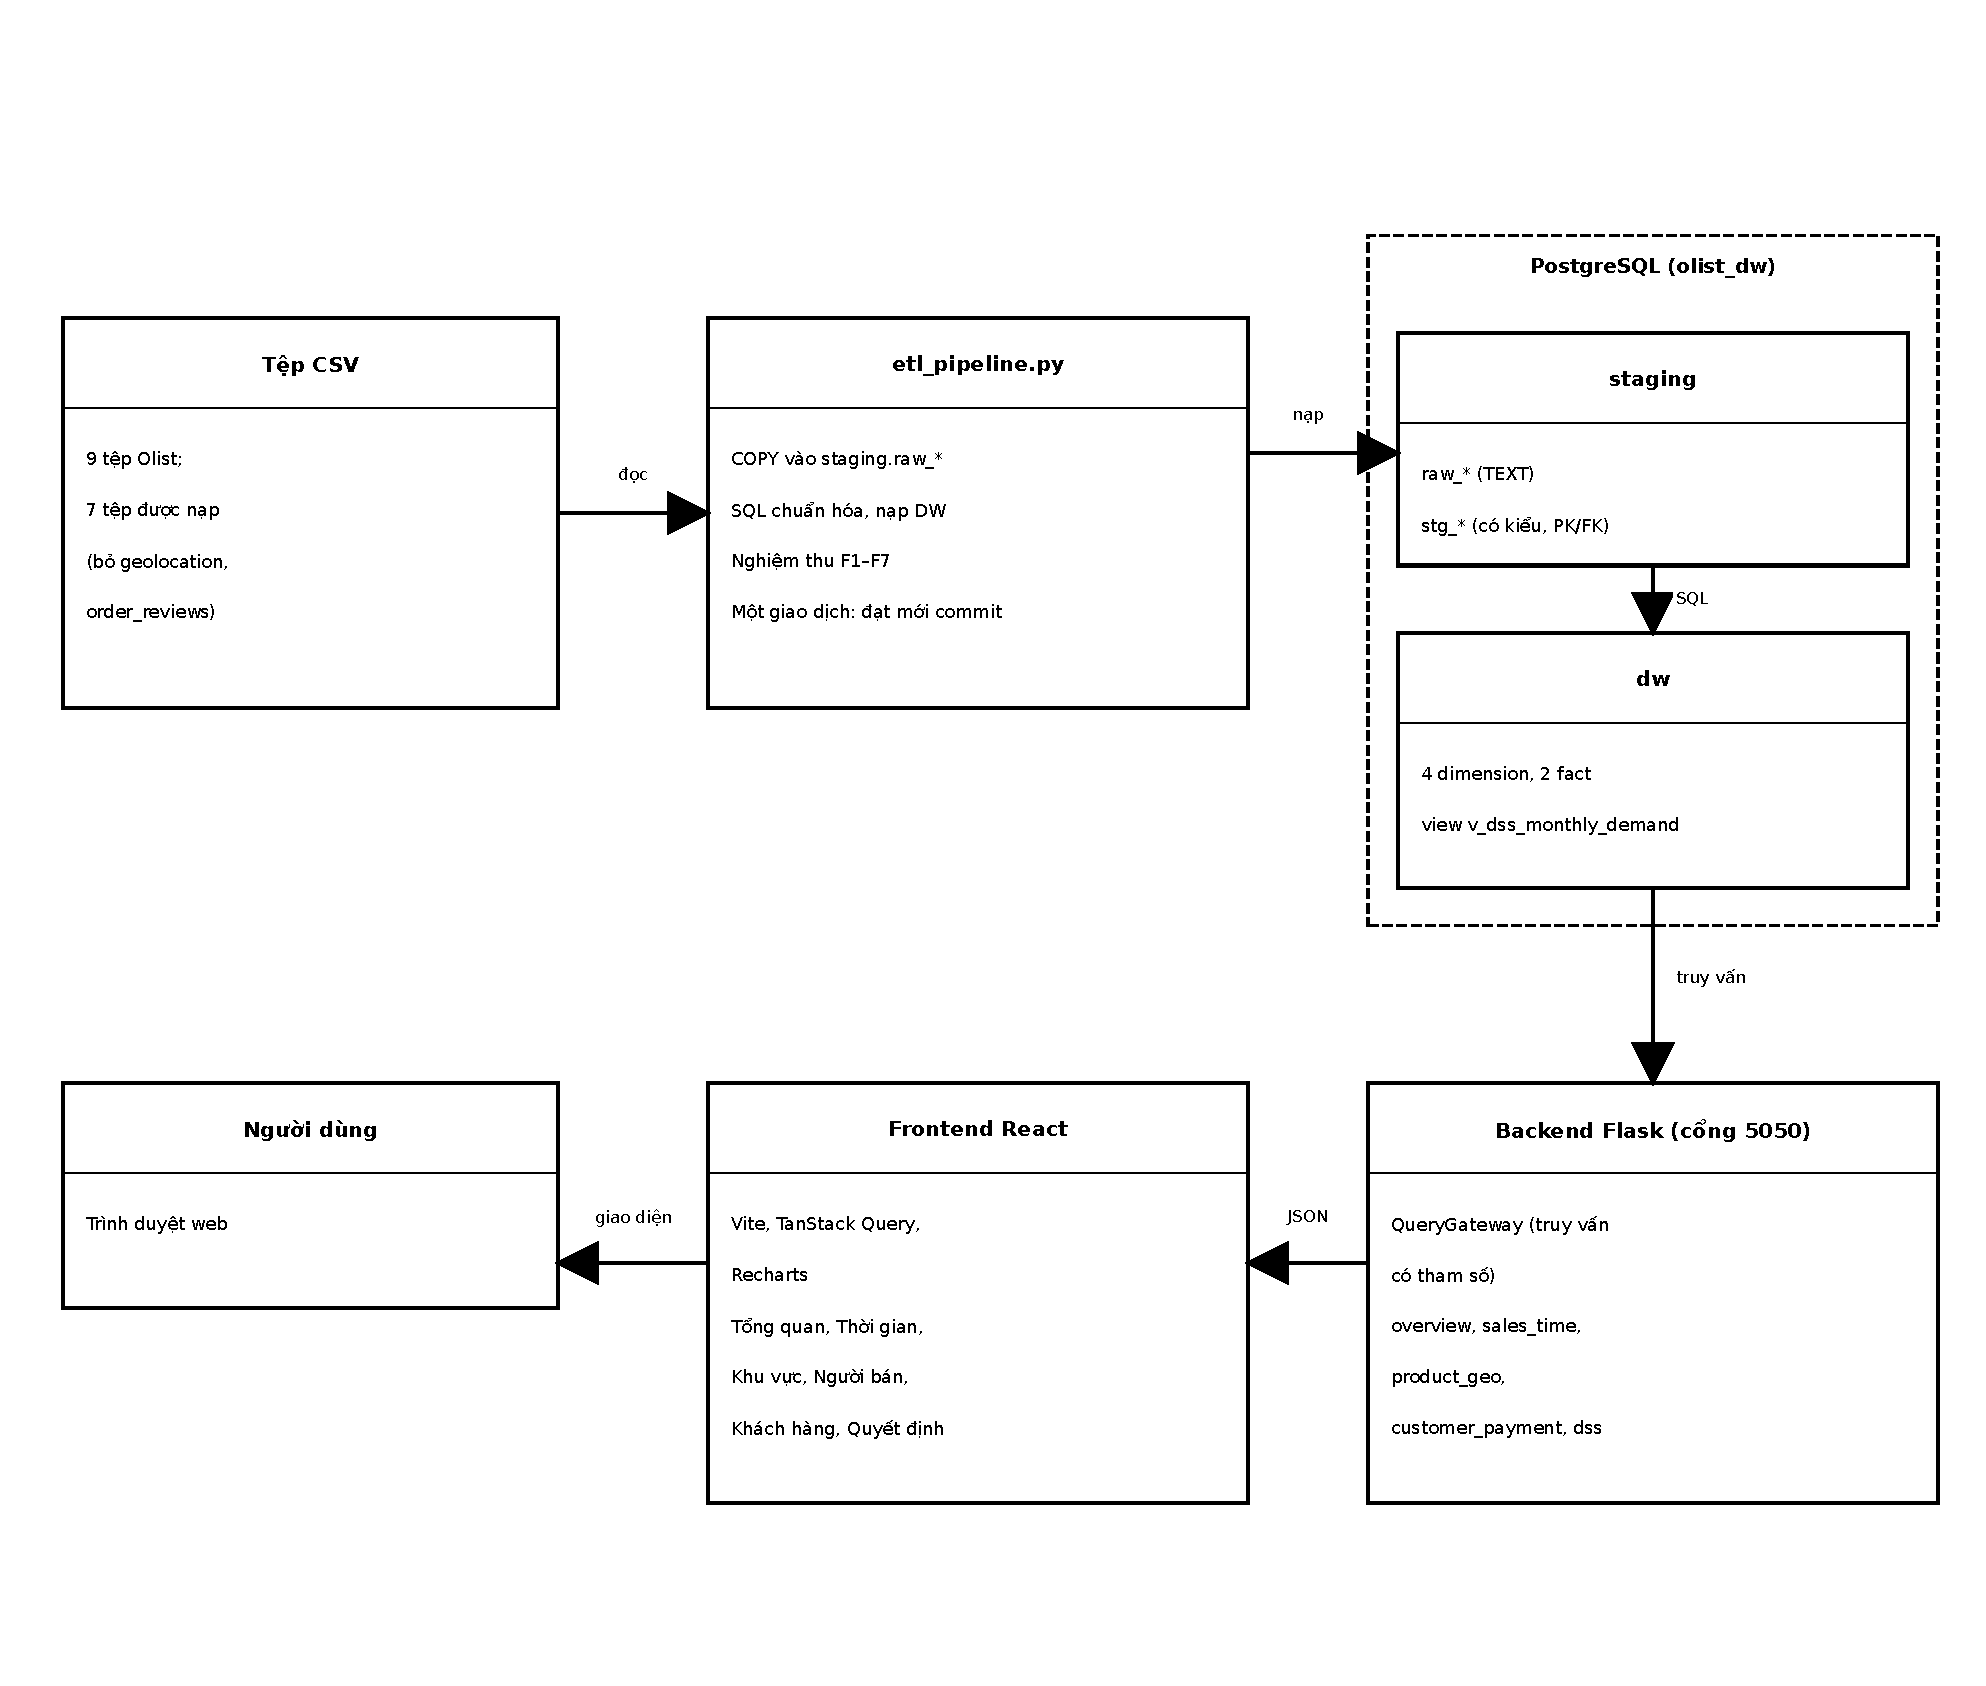
\includegraphics[width=\linewidth]{assets/fig_architecture.pdf}
\caption{Kiến trúc hệ thống}
\label{fig:architecture}
\end{figure}

Luồng xử lý gồm: (1) COPY các CSV vào \code{staging.raw_*} (toàn kiểu TEXT); (2) SQL chuẩn hóa sang \code{staging.stg_*} có kiểu và khóa; (3) SQL nạp \code{dw.dim_*} và hai bảng fact; (4) chạy bộ nghiệm thu; (5) tạo view nguồn cho DSS. Phép biến đổi chủ yếu diễn ra bằng SQL sau khi raw đã nằm trong PostgreSQL nên trình tự mang tính ELT; Python chỉ điều phối và nạp tệp bằng \code{copy_expert}. Backend Flask đọc kho qua một lớp truy vấn dùng chung; frontend React gọi API và vẽ biểu đồ.

\subsection{Công nghệ và cấu hình}
Backend dùng Flask, flask-cors và psycopg2; NumPy được dùng trong mô-đun dự báo DSS (cài kèm Pandas). SQLAlchemy và Pandas có trong \code{requirements.txt} vì \code{db_connect.py} dùng chung với các script chạy SQL, backend chỉ dùng hàm kết nối psycopg2 của tệp này. Lớp \code{QueryGateway} mở kết nối, thực thi truy vấn có tham số, chuyển kiểu kết quả sang JSON rồi đóng kết nối. API chạy ở cổng 5050. Frontend dùng React, TypeScript, Vite, TanStack Query, Recharts và Tailwind.

Kết nối cơ sở dữ liệu đọc từ tệp \code{.env} đặt cạnh \code{db_connect.py} (các biến \code{DB_HOST}, \code{DB_PORT}, \code{DB_NAME}, \code{DB_USER} và \code{DB_PASSWORD}). Chạy \code{python etl_pipeline.py} để nạp kho, rồi \code{python backend/run.py} và \code{npm run dev} trong \code{frontend}.

\clearpage\section{Mô hình đa chiều và Data Dictionary}
\subsection{Grain và mô hình vật lý}
Tên cột, kiểu, nullable và ràng buộc dưới đây lấy từ DDL của kho (\code{sql/dw/dw_schema.sql}) và của staging (\code{sql/staging/01_schema.sql}).

\code{dw.fact_sales} có grain một cặp (order\_id, order\_item\_id), với PK ghép đúng hai cột đó. Một sản phẩm có thể xuất hiện ở nhiều dòng cùng đơn nên grain không phải cặp (order, product). Hai measure vật lý là \code{price} và \code{freight_value}, kiểu \code{NUMERIC(10,2)}, NOT NULL và có CHECK không âm. Số món được tính bằng COUNT(*) trên các dòng hàng.

\code{dw.fact_customer_order} có grain một order\_id, giữ toàn bộ trạng thái, ngày mua, ngày duyệt, địa lý khách tại đơn và tổng thanh toán. \code{total_payment_value} là \code{NUMERIC(12,2)}, cho phép NULL; điều kiện CHECK chỉ chặn giá trị âm. Thanh toán được cộng theo đơn trước khi nối với fact, nhờ đó tránh tích chéo giữa nhiều dòng hàng và nhiều dòng thanh toán.

Mô hình là chòm sao fact (fact constellation) \cite{kimball} với dimension dùng chung, đồng thời có FK từ fact sales đến fact đơn. Đây không phải một Star Schema đơn lẻ độc lập, cũng không phải snowflake vì không có bảng dimension con. Sơ đồ hình~\ref{fig:physical} phản ánh nguyên trạng DDL, gồm cả cạnh fact--fact.

\begin{table}[H]\centering\small\renewcommand{\arraystretch}{1.15}
\begin{tabularx}{\linewidth}{p{3cm}YY}
\toprule Bảng dimension & Grain và khóa & Thuộc tính / vai trò\\\midrule
\code{dim_date} & Một ngày; PK date\_key=YYYYMMDD; full\_date UNIQUE & Năm, quý, tháng, ngày, thứ ISO, cuối tuần. Hai vai trò mua và duyệt.\\
\code{dim_customer} & Một customer\_unique\_id; customer\_key SERIAL PK & Business key CHAR(32), NOT NULL UNIQUE; không giữ thành phố/bang.\\
\code{dim_product} & Một product\_id; product\_key SERIAL PK & Business key CHAR(32), NOT NULL UNIQUE; danh mục gốc/Anh nullable.\\
\code{dim_seller} & Một seller\_id; seller\_key SERIAL PK & Business key CHAR(32), NOT NULL UNIQUE; không có địa lý seller.\\
\bottomrule\end{tabularx}
\caption{Các bảng dimension}
\end{table}

% Giữ trang sơ đồ ở khổ dọc theo yêu cầu, chấp nhận chữ trong hình nhỏ.
\clearpage
\begin{figure}[p]\centering
\sbox0{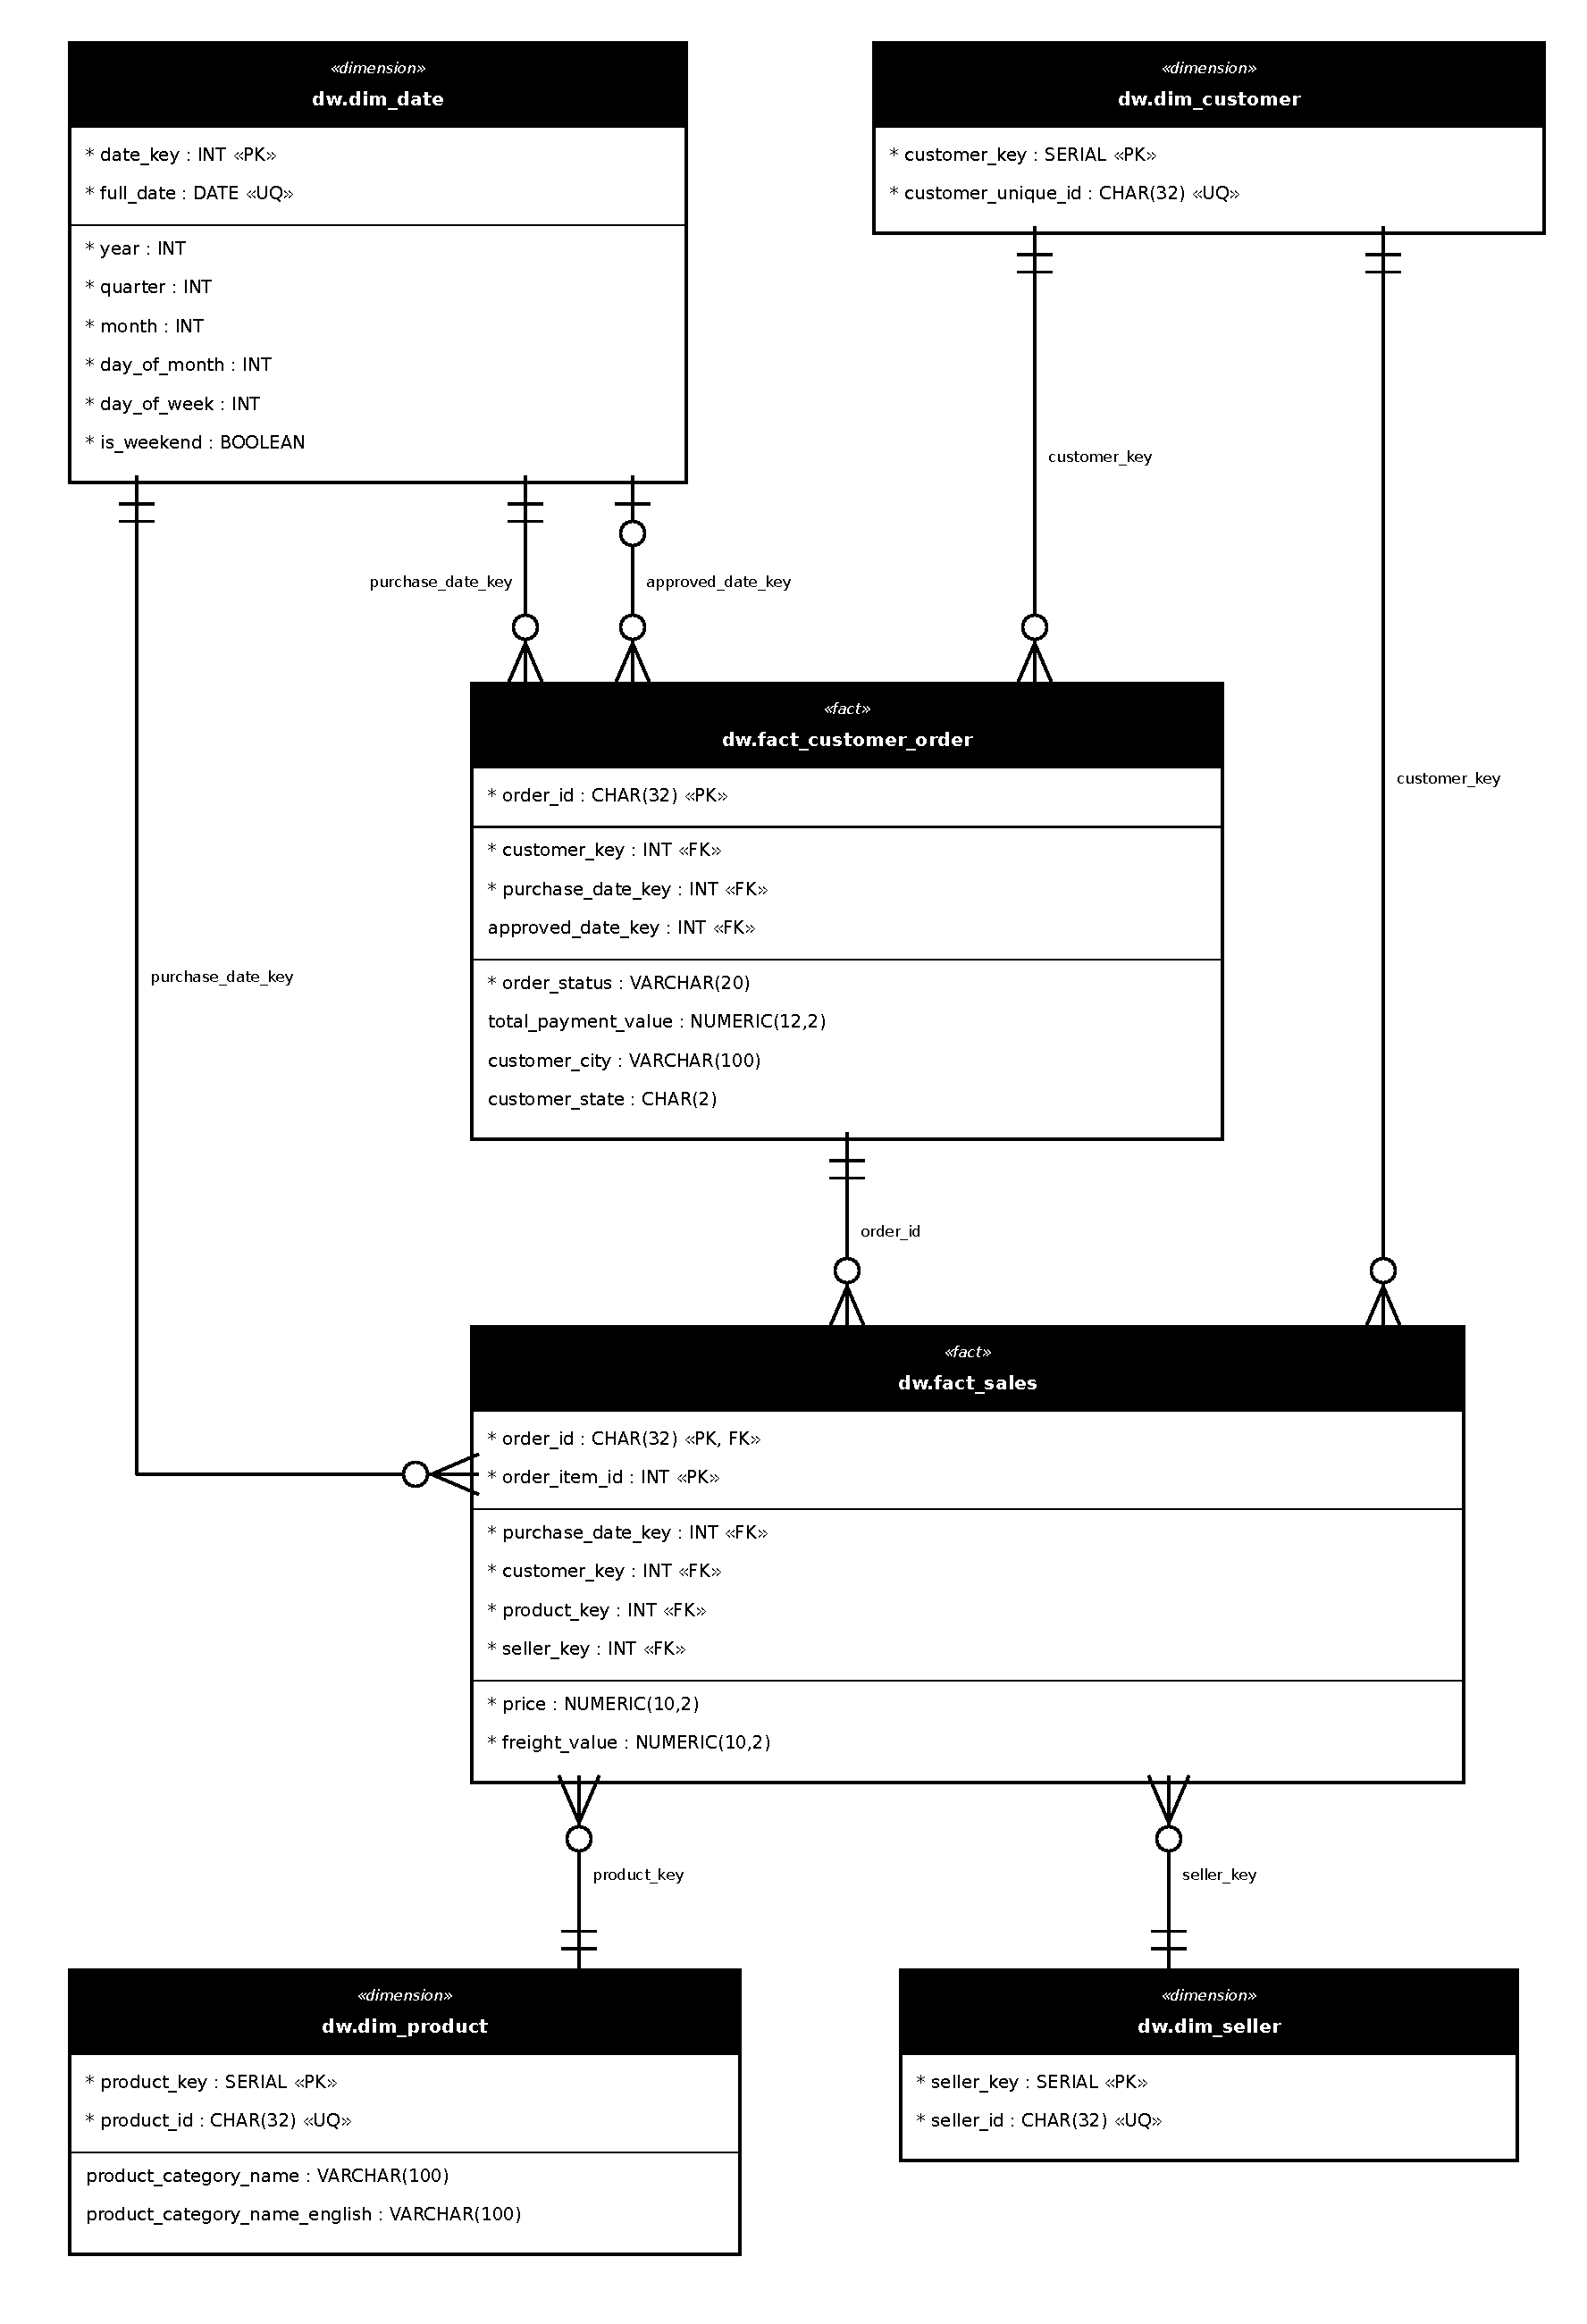
\includegraphics[width=\linewidth,height=0.83\textheight,keepaspectratio]{assets/fig_star_schema.pdf}}%
\setlength{\unitlength}{\wd0}%
\begin{picture}(1,1.4646)
\put(0,0){\usebox0}
\put(0.567,0.045){\sffamily\scriptsize Dấu * biểu diễn NOT NULL.}
\end{picture}
\caption{Mô hình vật lý của kho dữ liệu}
\label{fig:physical}
\end{figure}
\clearpage

\subsection{Quan hệ và khả năng cộng gộp}
Tất cả quan hệ DW là một--nhiều từ dimension sang fact, hoặc từ fact đơn sang fact sales. Mỗi dòng con có đúng một cha nếu FK bắt buộc; riêng \code{approved_date_key} nullable nên có 0 hoặc 1 ngày duyệt. DDL không bắt buộc một cha phải có ít nhất một con nên cardinality phía dòng con luôn là 0..N. Thực tế CSV có 775 đơn chưa có dòng hàng.

\code{purchase_date_key} và \code{customer_key} xuất hiện ở cả hai fact. Các FK riêng lẻ không tự bảo đảm chúng trùng khớp trên cùng \code{order_id}; script validate mới kiểm tra điều kiện này. Kho không dùng SCD Type 2, cột hiệu lực, thành viên ``unknown'' hay nạp tăng dần. Khóa SERIAL được sinh khi nạp nên không dùng làm định danh nghiệp vụ.

Tiền hàng và cước cộng được theo các chiều tại grain dòng sản phẩm. Tổng thanh toán chỉ cộng ở grain đơn hoặc sau khi gom mỗi đơn một lần; nối fact đơn với fact sales rồi SUM(total\_payment\_value) sẽ nhân bản tiền theo số dòng hàng. Số đơn riêng biệt không cộng được xuyên danh mục/seller; số khách riêng biệt không cộng được xuyên bang/năm. AOV và tỷ lệ phải tính lại từ tử số và mẫu số, không lấy trung bình đơn giản của các trung bình. Khi cần trạng thái hoặc địa lý đơn cho phân tích ở grain dòng hàng, truy vấn OLAP nối \code{fact_sales} với \code{fact_customer_order} trên \code{order_id} (quan hệ nhiều--một, không nhân bản dòng); các API màn Thời gian dùng phép nối này để lọc đơn delivered.

\subsection{Từ điển dữ liệu}
\begin{table}[H]\centering\small\renewcommand{\arraystretch}{1.1}
\begin{tabularx}{\linewidth}{p{3.5cm}p{2.9cm}Y}
\toprule Cột & Kiểu & Ý nghĩa\\\midrule
\multicolumn{3}{l}{dw.fact\_sales -- PK (order\_id, order\_item\_id)}\\
\code{order_id}, \code{order_item_id} & CHAR(32), INT & Định danh dòng hàng; FK \code{order_id} tới fact đơn.\\
\code{purchase_date_key} & INT & FK \code{dim_date}, ngày mua.\\
\code{customer_key}, \code{product_key}, \code{seller_key} & INT & FK tới ba dimension.\\
\code{price}, \code{freight_value} & NUMERIC(10,2) & Tiền hàng và cước của dòng; NOT NULL, $\geq 0$.\\
\midrule
\multicolumn{3}{l}{dw.fact\_customer\_order -- PK order\_id}\\
\code{customer_key} & INT & FK \code{dim_customer}.\\
\code{purchase_date_key}, \code{approved_date_key} & INT & FK \code{dim_date}; ngày duyệt có thể NULL.\\
\code{order_status} & VARCHAR(20) & Trạng thái đơn.\\
\code{total_payment_value} & NUMERIC(12,2) & Tổng thanh toán của đơn; NULL nếu không có dòng thanh toán, $\geq 0$.\\
\code{customer_city}, \code{customer_state} & VARCHAR, CHAR(2) & Địa lý khách tại thời điểm đặt đơn.\\
\bottomrule\end{tabularx}
\caption{Từ điển dữ liệu bảng fact}
\end{table}

Tầng raw giữ toàn bộ cột CSV kiểu TEXT, không khóa. Tầng staging có kiểu, PK/FK và chỉ giữ thuộc tính cần cho phân tích. Dữ liệu không có thông tin múi giờ nghiệp vụ nên ngày được lấy theo giá trị trong CSV.

\clearpage\section{Quy trình nạp và kiểm soát chất lượng}
\subsection{Nạp raw và chuẩn hóa sang staging}
\code{etl_pipeline.py} đảm bảo database tồn tại, tạo schema \code{staging}, rồi COPY bảy tệp CSV vào \code{staging.raw_*} (HEADER, UTF8; toàn TEXT để tách việc đọc dữ liệu khỏi ép kiểu). Chế độ mặc định tạo lại staging và DW; tùy chọn \code{--reload-only} giữ schema và truncate rồi nạp lại, không phải nạp tăng dần.

\code{03_promote.sql} chuyển raw sang \code{staging.stg_*} bằng cách btrim định danh và chuỗi, dùng NULLIF để đổi chuỗi rỗng thành NULL, rồi ép kiểu timestamp, integer, numeric. Bước này không khử trùng lặp, không nội suy giá trị thiếu và không sửa số tiền; PK/FK và kiểu sẽ làm INSERT thất bại nếu dữ liệu không phù hợp. Pipeline in số dòng từng bảng staging để phát hiện mất dòng.

Thông tin giao hàng, kích thước sản phẩm, vị trí seller, loại thanh toán và số kỳ trả góp được bỏ khỏi staging có kiểu theo nhu cầu phân tích hiện có; do đó DW không hỗ trợ SLA giao hàng hay phân tích loại thanh toán.

\subsection{Nạp dimension trước fact}
\begin{enumerate}[leftmargin=*]
\item \code{dim_date}: sinh lịch liên tục từ ngày nhỏ nhất đến lớn nhất của ngày mua và ngày duyệt (mọi trạng thái); thứ và cuối tuần tính theo ISO.
\item \code{dim_customer}: DISTINCT theo \code{customer_unique_id}; \code{dim_product}: LEFT JOIN bản dịch danh mục; \code{dim_seller}: theo \code{seller_id}.
\item \code{fact_customer_order}: gom thanh toán theo \code{order_id} trước rồi LEFT JOIN; đơn không có payment giữ NULL, không thay bằng 0.
\item \code{fact_sales}: nối dòng hàng với đơn, khách và các dimension; lấy ngày mua và khách từ cùng đơn.
\end{enumerate}

\begin{table}[H]\centering\small
\begin{tabularx}{\linewidth}{p{3.7cm}YY}
\toprule Đích & Nguồn chính & Quy tắc đáng chú ý\\\midrule
\code{dim_customer} & stg\_customers & DISTINCT customer\_unique\_id, không phải customer\_id.\\
\code{dim_product} & stg\_products, bản dịch & LEFT JOIN; thiếu bản dịch vẫn giữ sản phẩm.\\
\code{fact_customer_order} & stg\_orders, customers, payments & Tổng tiền gom trước khi nối; địa lý theo customer\_id của đơn.\\
\code{fact_sales} & stg\_order\_items và các dimension & Giữ grain dòng hàng; không nối trực tiếp payment.\\
\bottomrule\end{tabularx}
\caption{Ánh xạ staging sang DW}
\end{table}

\subsection{Nghiệm thu dữ liệu}
Bộ nghiệm thu nằm ở \code{sql/dw/03_validate.sql}, chạy ngay sau khi nạp; mỗi tiêu chí sai sẽ \code{RAISE EXCEPTION}, pipeline dừng và toàn bộ lần nạp bị rollback. Các tiêu chí kiểm tra bất biến của dữ liệu, không gõ cứng số đếm của một bản dữ liệu cụ thể:

\begin{table}[H]\centering\small
\begin{tabularx}{\linewidth}{lY}
\toprule Nhóm & Nội dung kiểm tra\\\midrule
F1 & Tổng tiền hàng và cước ở \code{fact_sales} bằng tổng ở staging.\\
F2 & Không trùng cặp (order\_id, order\_item\_id); mọi đơn của \code{fact_sales} có trong fact đơn; ngày mua và khách khớp giữa hai fact.\\
F3 & Khóa ngoại tới các dimension đều ánh xạ được.\\
F4 & Tổng thanh toán theo đơn khớp staging; đơn có thanh toán NULL thì nguồn thực sự không có dòng thanh toán (số đơn như vậy chỉ được báo, không bắt buộc bằng một giá trị).\\
F5 & Số đơn theo từng trạng thái khớp giữa staging và fact.\\
F6 & Các cột của \code{dim_date} nhất quán với \code{full_date}.\\
F7 & Không có giá hoặc cước âm; không có khóa bắt buộc bị NULL.\\
\bottomrule\end{tabularx}
\caption{Tiêu chí nghiệm thu F1--F7}
\end{table}

Có thể chạy lại bộ nghiệm thu mà không nạp lại dữ liệu bằng \code{check_acceptance.py}; script thoát mã 1 khi có tiêu chí sai. Các phép so sánh dùng \code{IS DISTINCT FROM} nên bắt được cả trường hợp một vế NULL. Một phép thử làm rỗng \code{fact_sales} trong giao dịch rồi hủy cho thấy bản dùng \code{<>} vẫn báo đạt (vì tổng tiền là NULL), còn bản hiện tại báo lỗi F1.

\subsection{Giao dịch và khả năng tái lập}
Toàn bộ pipeline (tạo schema, nạp raw, promote, tạo và nạp DW, nghiệm thu, tạo view DSS) chạy trong một giao dịch PostgreSQL và chỉ \code{COMMIT} khi mọi bước thành công. Lỗi ở bất kỳ bước nào làm giao dịch bị rollback, nên một lần chạy lại thất bại vẫn giữ nguyên kho cũ. Điều này đã được kiểm tra bằng cách giả lập lỗi ở bước nghiệm thu, khi đó pipeline dừng và \code{fact_sales} vẫn giữ 112.650 dòng, view DSS vẫn tồn tại.

Chế độ mặc định xóa schema rồi tạo lại nên cho cùng kết quả sau mỗi lần chạy; \code{--reload-only} không RESTART IDENTITY nên khóa thay thế có thể khác và không được dùng làm định danh nghiệp vụ. Vì tạo lại schema \code{dw} xóa cả các view, bước cuối của pipeline tạo lại view \code{dw.v_dss_monthly_demand} (mục~\ref{sec:dss-data}). Pipeline đã được chạy đầy đủ trên PostgreSQL 16 và đạt F1--F7 (chương~\ref{sec:results}).

\clearpage\section{Phân tích OLAP và giao diện}\label{sec:olap}
\subsection{Định nghĩa KPI nhất quán theo grain}
Gọi $D$ là tập đơn delivered và $I(D)$ là các dòng hàng thuộc tập đó. Các thước đo dùng xuyên suốt các màn hình là:
\begin{align}
\text{Doanh thu hàng} &= \sum_{i\in I(D)} price_i, &
\text{Cước} &= \sum_{i\in I(D)} freight_i,\\
\text{Thanh toán} &= \sum_{o\in D,\,payment_o\ne NULL} payment_o,\\
\mathrm{AOV} &= \frac{\text{Thanh toán}}{\#\{o\in D: payment_o\ne NULL\}}.
\end{align}
Số đơn và số dòng hàng là hai đại lượng khác nhau. Khi thống kê khách, dùng \code{customer_unique_id}, không đếm \code{customer_id}. Tỷ lệ mua lại bằng số khách có ít nhất hai đơn delivered chia tổng số khách có đơn delivered. Thanh toán chỉ cộng ở grain đơn; ví dụ truy vấn dưới đây lấy từ trang Tổng quan:
\begin{lstlisting}[language=SQL]
SELECT count(*) AS orders,
       count(total_payment_value) AS paid_orders,
       sum(total_payment_value) AS payment,
       avg(total_payment_value) AS aov
FROM dw.fact_customer_order
WHERE order_status = 'delivered';
\end{lstlisting}
Các thước đo đếm riêng biệt (số đơn, số khách) không cộng được xuyên danh mục, seller hay bang vì một đơn có thể chứa nhiều danh mục hoặc seller; AOV và tỷ lệ luôn tính lại từ tử số và mẫu số.

\subsection{Các thao tác OLAP theo từng màn hình}
Phần này mô tả những gì người dùng thực hiện được trên giao diện; mỗi thao tác là một lời gọi API riêng đến kho.

\begin{table}[H]\centering\small\renewcommand{\arraystretch}{1.15}
\begin{tabularx}{\linewidth}{p{2.3cm}YY}
\toprule Màn hình & Thao tác OLAP & Cách thực hiện trên giao diện\\\midrule
Tổng quan & Bốn thẻ KPI; xu hướng tháng; top danh mục & Doanh thu hàng, giá trị đơn trung bình, số khách kèm tỷ lệ mua lại, cước kèm tỷ lệ so với doanh thu hàng.\\
Thời gian & Drill-down / roll-up, slice, dice, pivot & Bộ lọc phân cấp Năm $\rightarrow$ Quý $\rightarrow$ Tháng $\rightarrow$ Ngày; nhấn cột để đi xuống, nút lên để gộp lại; chế độ nhiều năm (dice) và chế độ Tháng $\times$ Năm (pivot).\\
Khu vực & Drill-down, slice & Bang $\rightarrow$ thành phố; chọn bang thì danh mục lọc theo bang; slice theo năm, quý.\\
Người bán & Xếp hạng, slice, dice & Top 5/10/20 người bán theo danh mục, bang, kỳ; ``khối'' người bán $\times$ danh mục $\times$ bang.\\
Khách hàng & Drill-down, dice, ma trận, xếp hạng & Ba chiều: nhóm khách, địa lý, trạng thái đơn; dice theo nhiều bang và khoảng năm; ma trận bang $\times$ năm; top khách theo bang.\\
\bottomrule\end{tabularx}
\caption{Thao tác OLAP theo màn hình}
\end{table}

Màn Tổng quan (hình~\ref{fig:ui-overview}) gom bốn thẻ KPI và bốn biểu đồ thu nhỏ, mỗi biểu đồ có nút mở sang màn chi tiết tương ứng. Biểu đồ thời gian ở đây chỉ hiện doanh thu theo tháng; tăng trưởng được xem ở màn Thời gian.

\begin{figure}[H]\centering
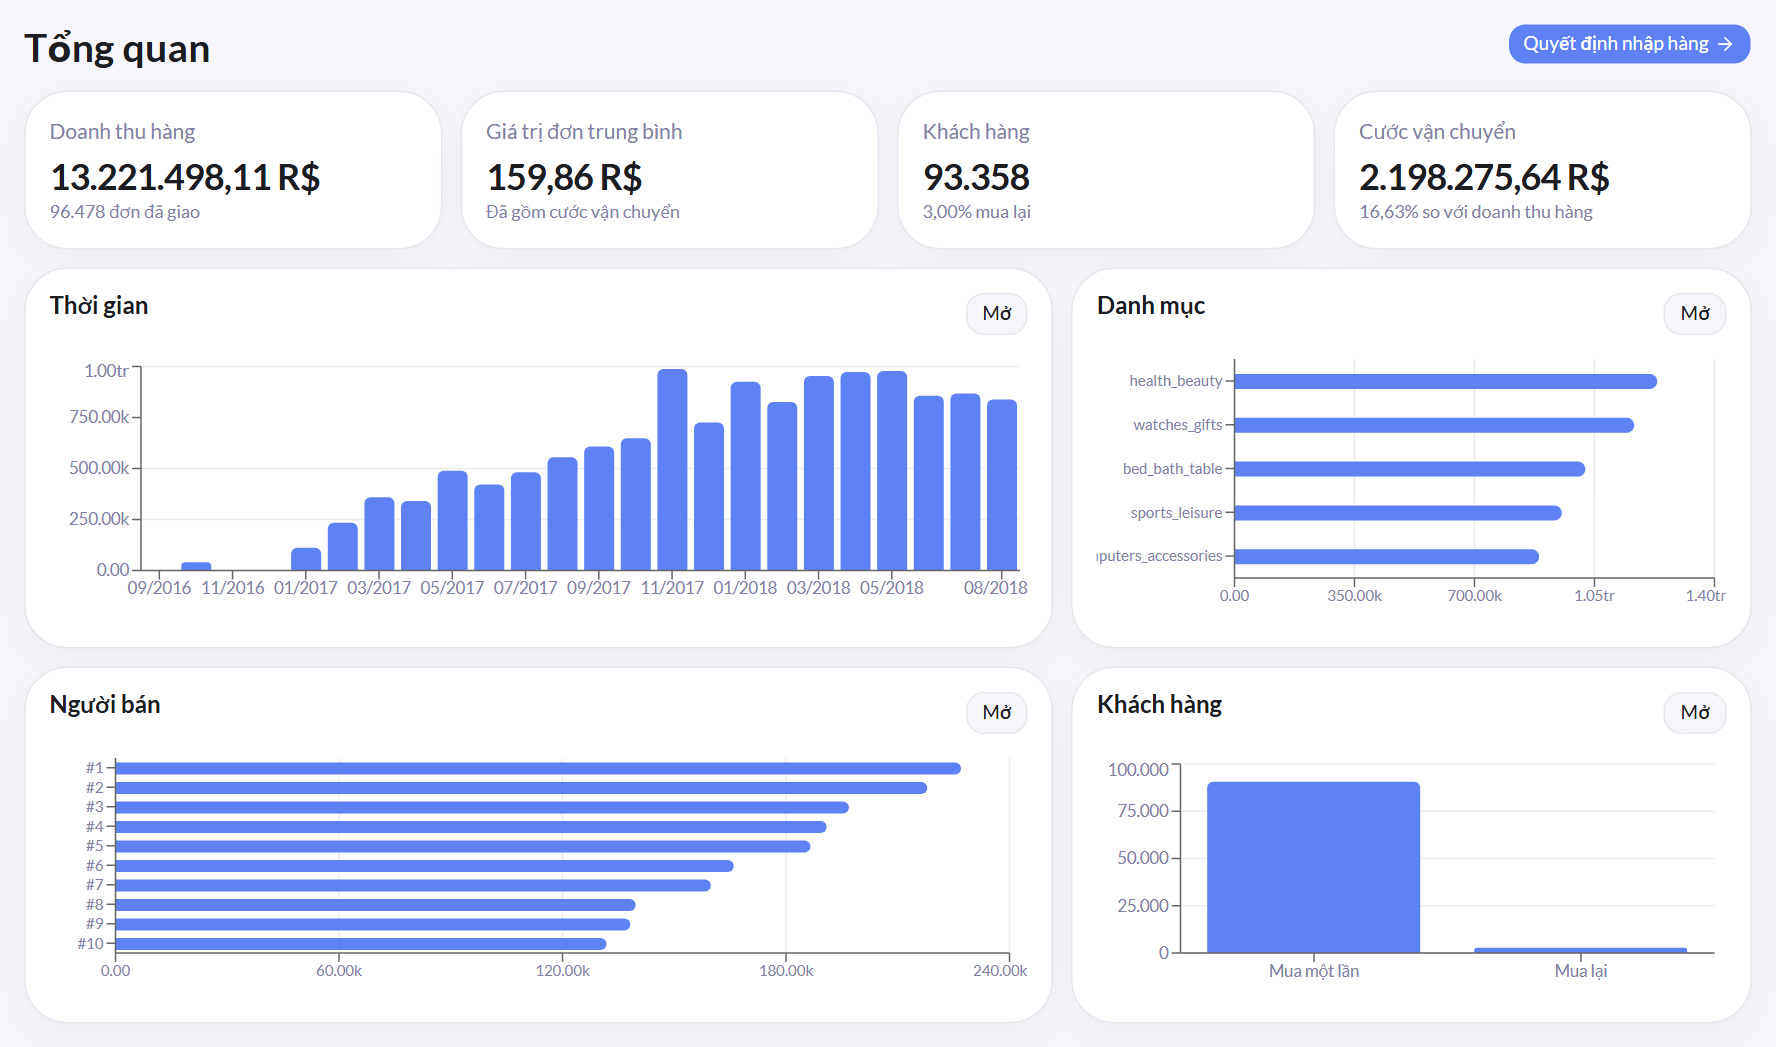
\includegraphics[width=\linewidth,height=0.42\textheight,keepaspectratio]{assets/ui_overview.png}
\caption{Màn Tổng quan}\label{fig:ui-overview}
\end{figure}


\subsubsection*{Màn Thời gian}
Chọn một trong ba thước đo: Doanh thu, Phí vận chuyển, Số lượng sản phẩm. Ở cấp năm và quý, bảng kèm tăng trưởng YoY và QoQ cùng kỳ, nghĩa là chỉ so các tháng có dữ liệu ở cả hai kỳ. Cách này cần thiết vì dữ liệu delivered chỉ phủ từ 09/2016 đến 08/2018 và thiếu 11/2016; chia tổng cả năm cho tổng cả năm trước sẽ trộn tăng trưởng thật với số tháng chênh lệch. Ví dụ 2018 (tháng 1--8) so với cùng các tháng của 2017 tăng +141,13\%, trong khi so với cả 12 tháng 2017 chỉ ra +21,05\%. Bảng cũng ghi số tháng có dữ liệu và số tháng dùng để so sánh. Ở cấp tháng, bảng hiển thị MoM; LAG được tính trên toàn chuỗi trước khi lọc nên tháng đầu của một kỳ vẫn có giá trị so sánh.

Ba loại tăng trưởng này dùng chung một quy tắc để loại các tháng gần như trống. Hai tháng 09/2016 (134,97 R\$) và 12/2016 (10,90 R\$) chỉ bằng 0,00--0,06\% trung vị nên không được dùng làm mốc so sánh. Một tháng bị coi là quá thưa khi nhỏ hơn 1\% trung vị các tháng có dữ liệu của cùng thước đo. MoM để trống khi tháng trước quá thưa, nên 10/2016 và 01/2017 không có MoM thay vì những con số vô nghĩa như +1.025.573\% làm trục biểu đồ giãn ra. Với QoQ và YoY, một cặp tháng cùng vị trí ở hai kỳ chỉ được đem so khi cả hai tháng đều đạt ngưỡng. Vì vậy Q1/2017 chỉ so 01/2017 với 10/2016 và tăng 177,24\% thay vì 1.067,68\%, còn Q4/2016 không còn cặp nào để so nên để trống.

Riêng YoY còn một điều kiện nữa là phải có ít nhất 3 cặp tháng hợp lệ, nếu không thì để trống. Lý do là tăng trưởng của cả một năm mà chỉ dựa trên một hoặc hai tháng thì không còn là so sánh theo năm, mà chỉ là tăng trưởng của vài tháng lẻ. Trên dữ liệu thật, YoY của 2017 so với 2016 chỉ có một cặp hợp lệ (10/2017 với 10/2016, tăng khoảng +1.507\%, một con số lớn vì mốc so sánh còn rất nhỏ) nên để trống, thay vì +4.796\% khi ghép cả các tháng gần như trống. YoY của 2018 có 8 cặp (tháng 1--8) nên vẫn là +141,13\%. Mức 3 tháng tương đương một quý, đơn vị nhỏ nhất của các so sánh theo kỳ trên màn này. Cột số tháng so cùng kỳ cho người đọc thấy mỗi kỳ dựa trên bao nhiêu tháng; QoQ không đặt điều kiện này nên Q1/2017 vẫn hiển thị kèm số 1.

Ngưỡng được đặt theo trung vị vì trung vị không bị kéo lệch bởi chính các tháng gần như trống ở đầu chuỗi, tháng Black Friday 11/2017 hay đà tăng mạnh từ 2017 sang 2018, trong khi trung bình chịu ảnh hưởng của các giá trị này. Ngưỡng cũng là tỷ lệ so với trung vị của từng thước đo nên dùng chung được cho doanh thu, cước (R\$) và số món mà không cần đặt một ngưỡng tuyệt đối riêng cho mỗi đơn vị. Mức 1\% không nhạy vì tháng thật nhỏ nhất (10/2016) đã bằng khoảng 6,5\% trung vị, nên mọi ngưỡng từ 0,1\% đến 6\% cho cùng kết quả. Báo cáo không nâng ngưỡng lên khoảng 10\% chỉ để bỏ nốt tháng 10/2016, vì mức đó chỉ cách tháng 01/2017 (khoảng 17--19\% trung vị) chưa đến 3 lần và trông như chỉnh ngưỡng cho khớp một tháng; điều kiện số tháng tối thiểu của YoY có lý do riêng nên được dùng thay thế.

Chế độ nhiều năm (dice) gộp theo năm, quý, tháng hoặc ngày trong một khoảng năm, với bộ lọc quý, tháng và loại ngày (cuối tuần hay ngày thường). Chế độ pivot và nút ma trận hiển thị biểu đồ cùng bảng Tháng $\times$ Năm. Tháng không có giao dịch để trống thay vì ghi 0, để không tạo mức giảm giả.

Hình~\ref{fig:ui-time} là màn Thời gian ở cấp năm, bảng bên dưới cho thấy tăng trưởng cùng kỳ cùng số tháng dùng để so sánh; hình~\ref{fig:ui-pivot} là chế độ pivot Tháng $\times$ Năm, gồm biểu đồ cột theo năm và bảng ma trận tương ứng.

\begin{figure}[H]\centering
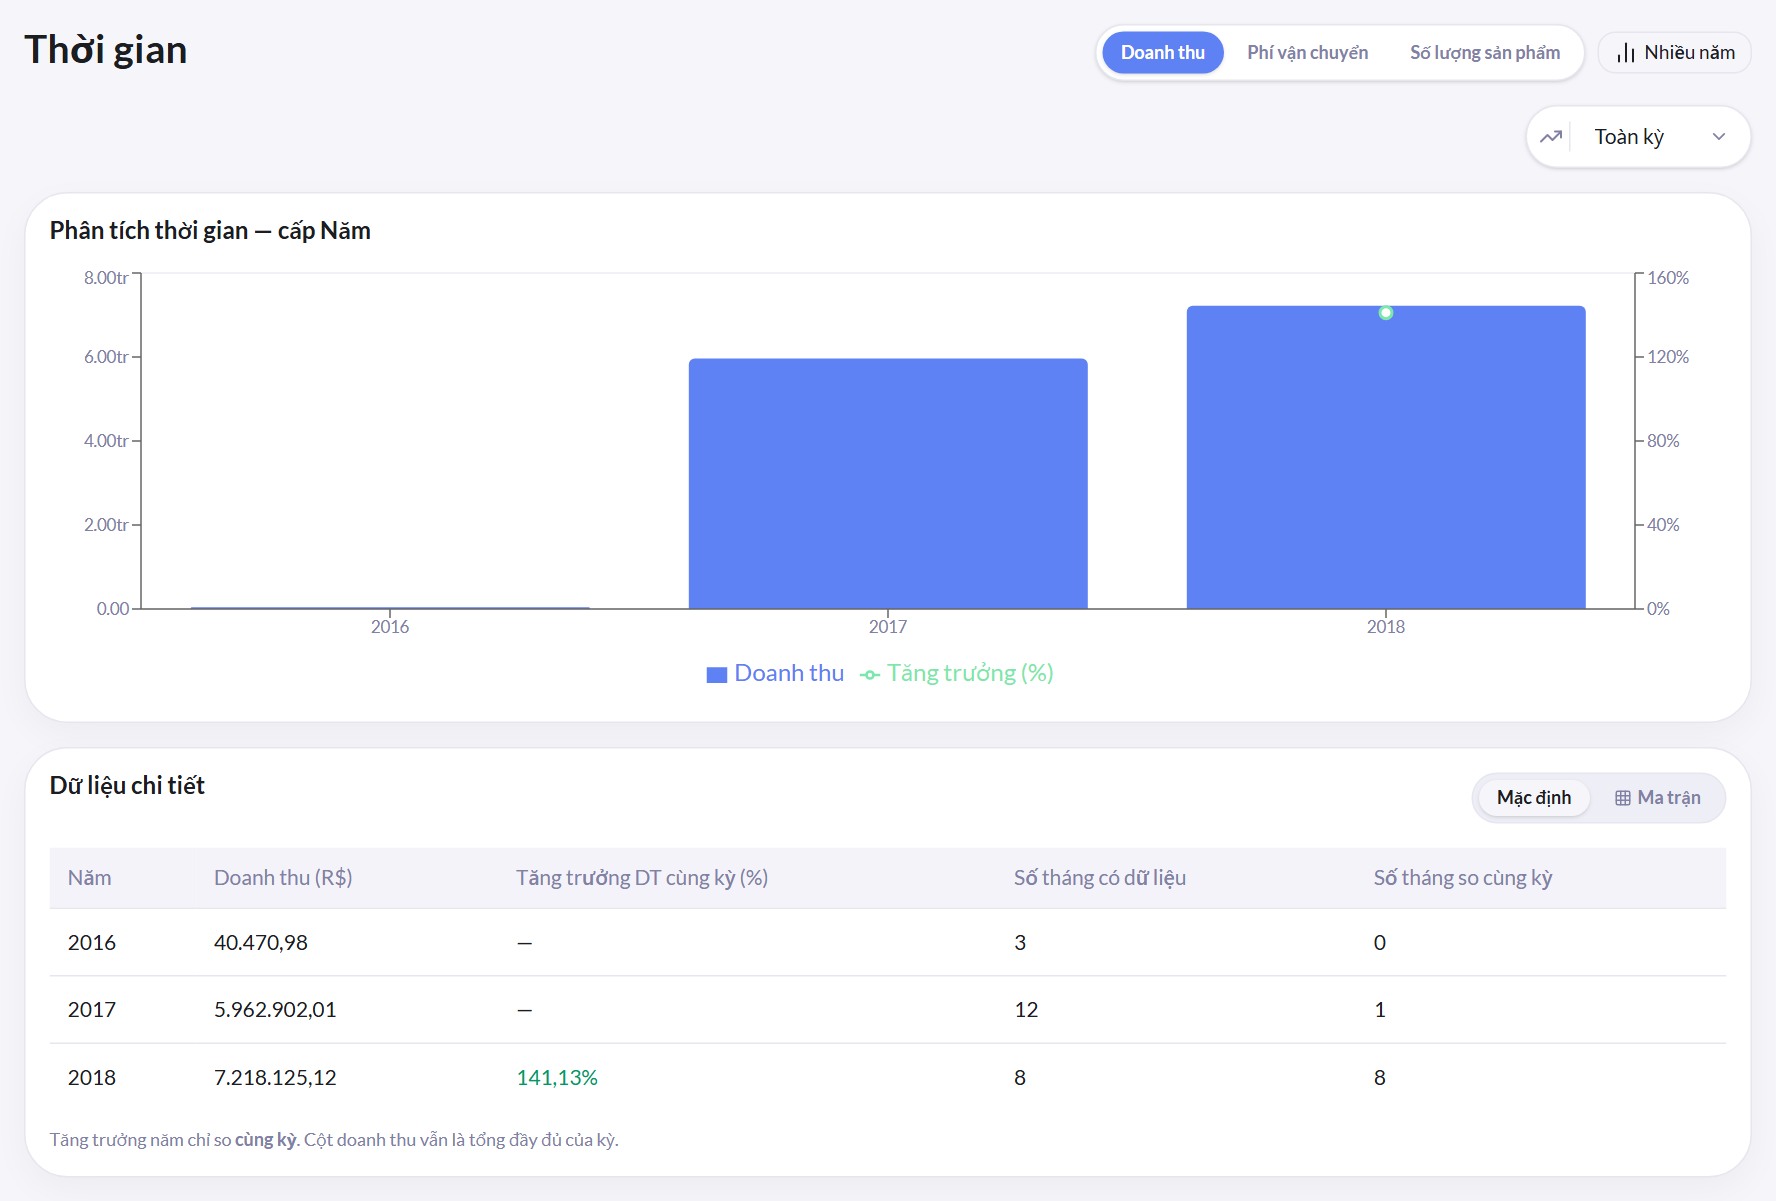
\includegraphics[width=\linewidth,height=0.42\textheight,keepaspectratio]{assets/ui_time.png}
\caption{Màn Thời gian ở cấp năm}\label{fig:ui-time}
\end{figure}

\begin{figure}[H]\centering
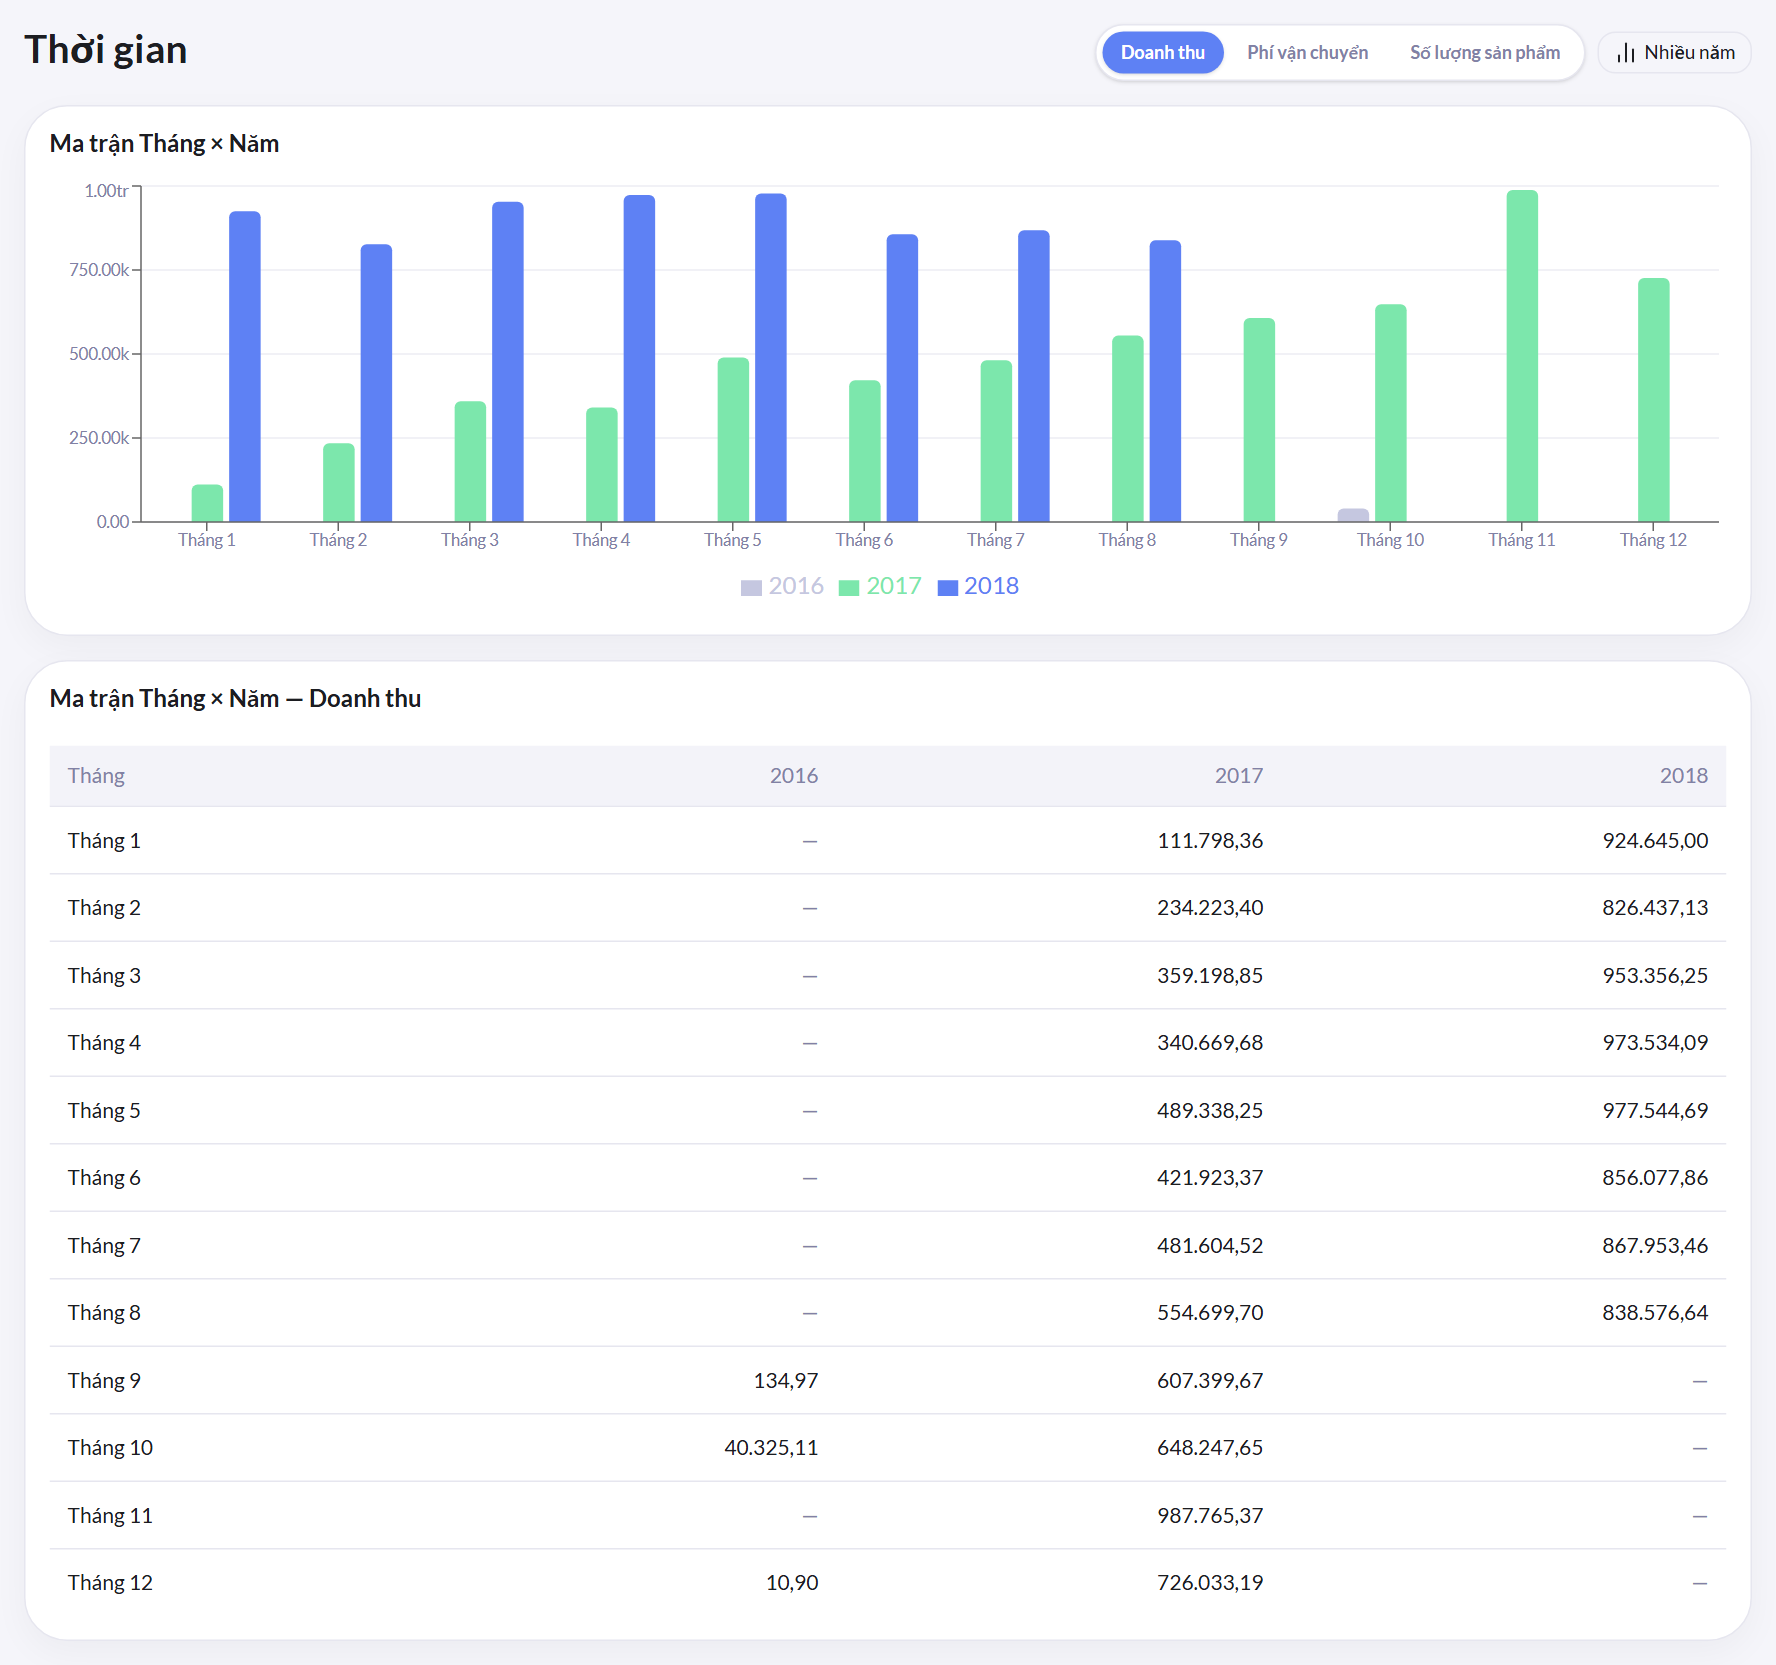
\includegraphics[width=\linewidth,height=0.5\textheight,keepaspectratio]{assets/ui_time_pivot.png}
\caption{Pivot Tháng $\times$ Năm}\label{fig:ui-pivot}
\end{figure}

\subsubsection*{Màn Khu vực và Người bán}
Màn Khu vực hiển thị doanh thu, cước, tỷ lệ cước/giá và số đơn; bảng bang chuyển sang thành phố của bang được chọn và danh mục được lọc theo bang. Bộ lọc năm và quý là thao tác slice. Màn Người bán xếp hạng top 5, 10 hoặc 20 người bán, lọc theo danh mục và bang khách; nút ``Xem khối'' dựng khối người bán $\times$ danh mục $\times$ bang cho nhiều danh mục và nhiều bang, với tổng theo bang và theo danh mục, và cho phép lấy một người bán, bang hoặc danh mục làm lát cắt. Địa lý trong cả hai màn là nơi khách đặt đơn, không phải nơi người bán.

Hình~\ref{fig:ui-geo} là màn Khu vực ở toàn kỳ, còn hình~\ref{fig:ui-cube} là khối người bán khi chọn ba danh mục health\_beauty, watches\_gifts, bed\_bath\_table và ba bang SP, RJ, MG.

\begin{figure}[H]\centering
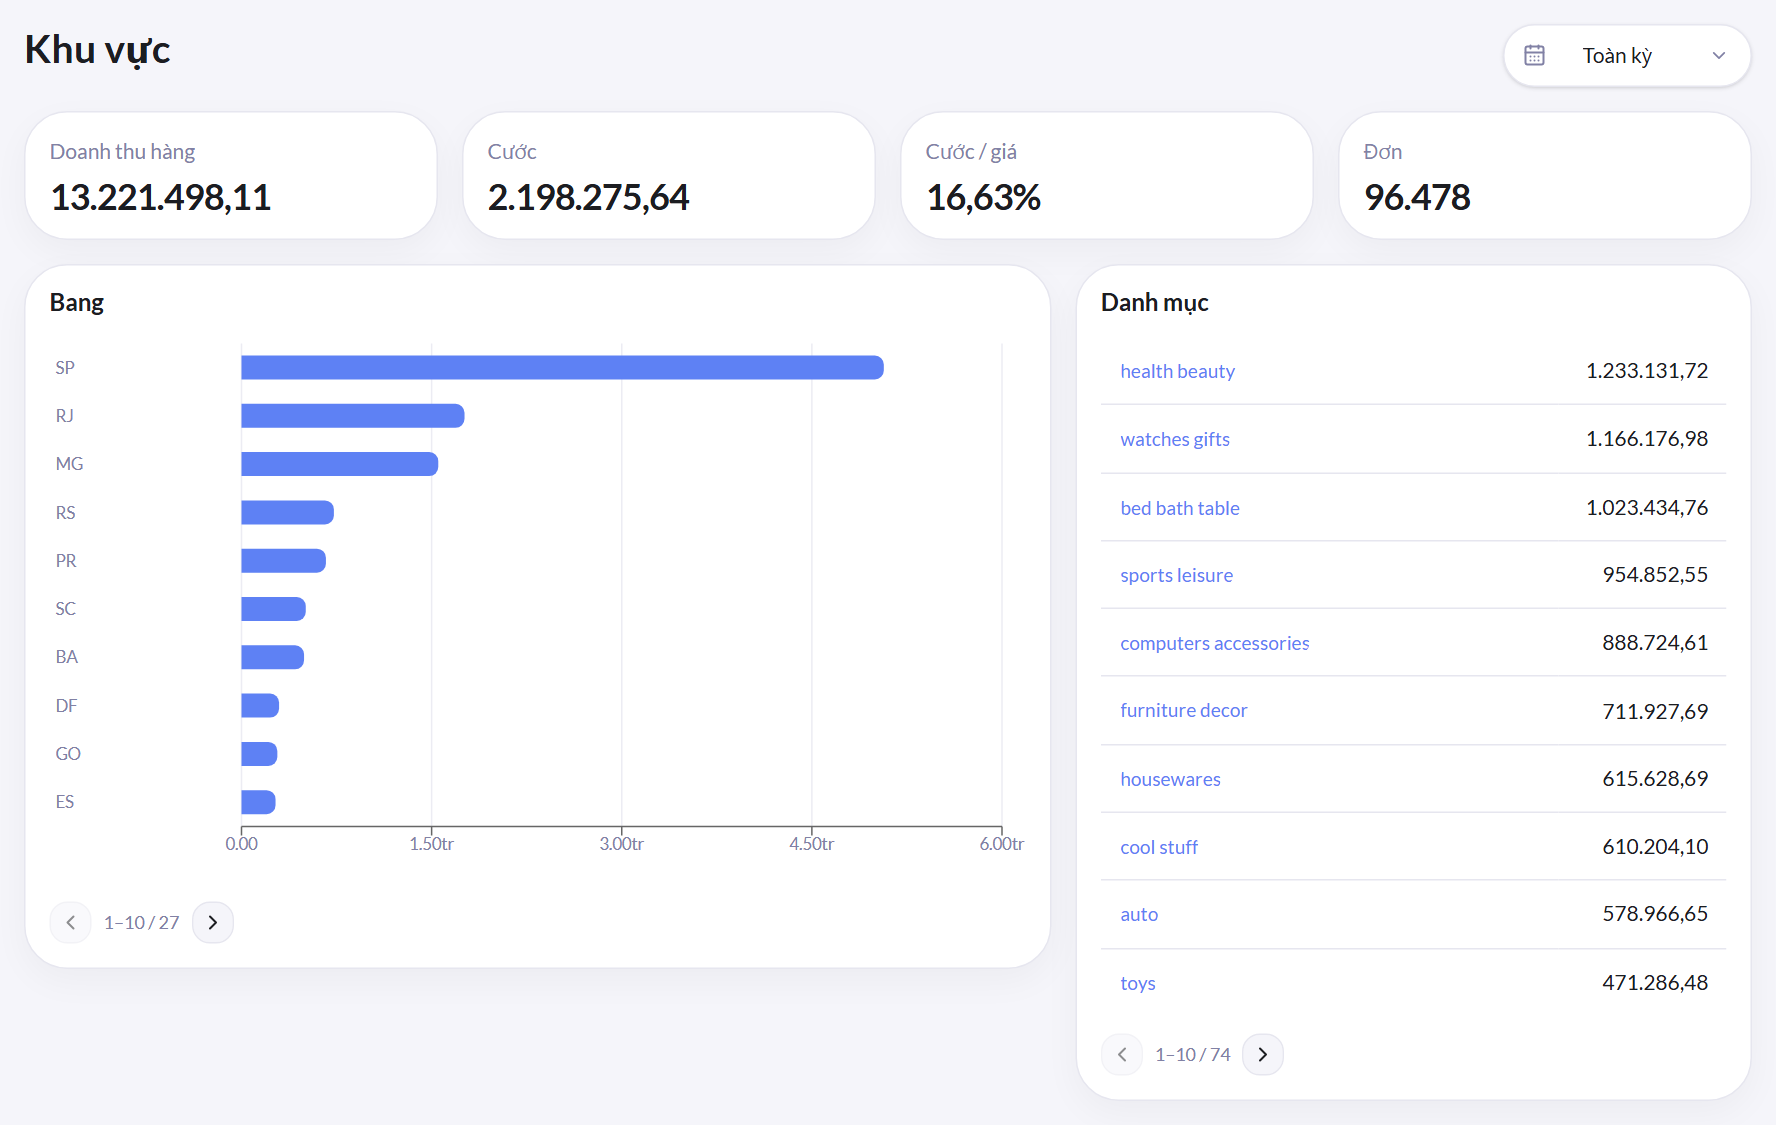
\includegraphics[width=\linewidth,height=0.42\textheight,keepaspectratio]{assets/ui_geo.png}
\caption{Màn Khu vực}\label{fig:ui-geo}
\end{figure}

\begin{figure}[H]\centering
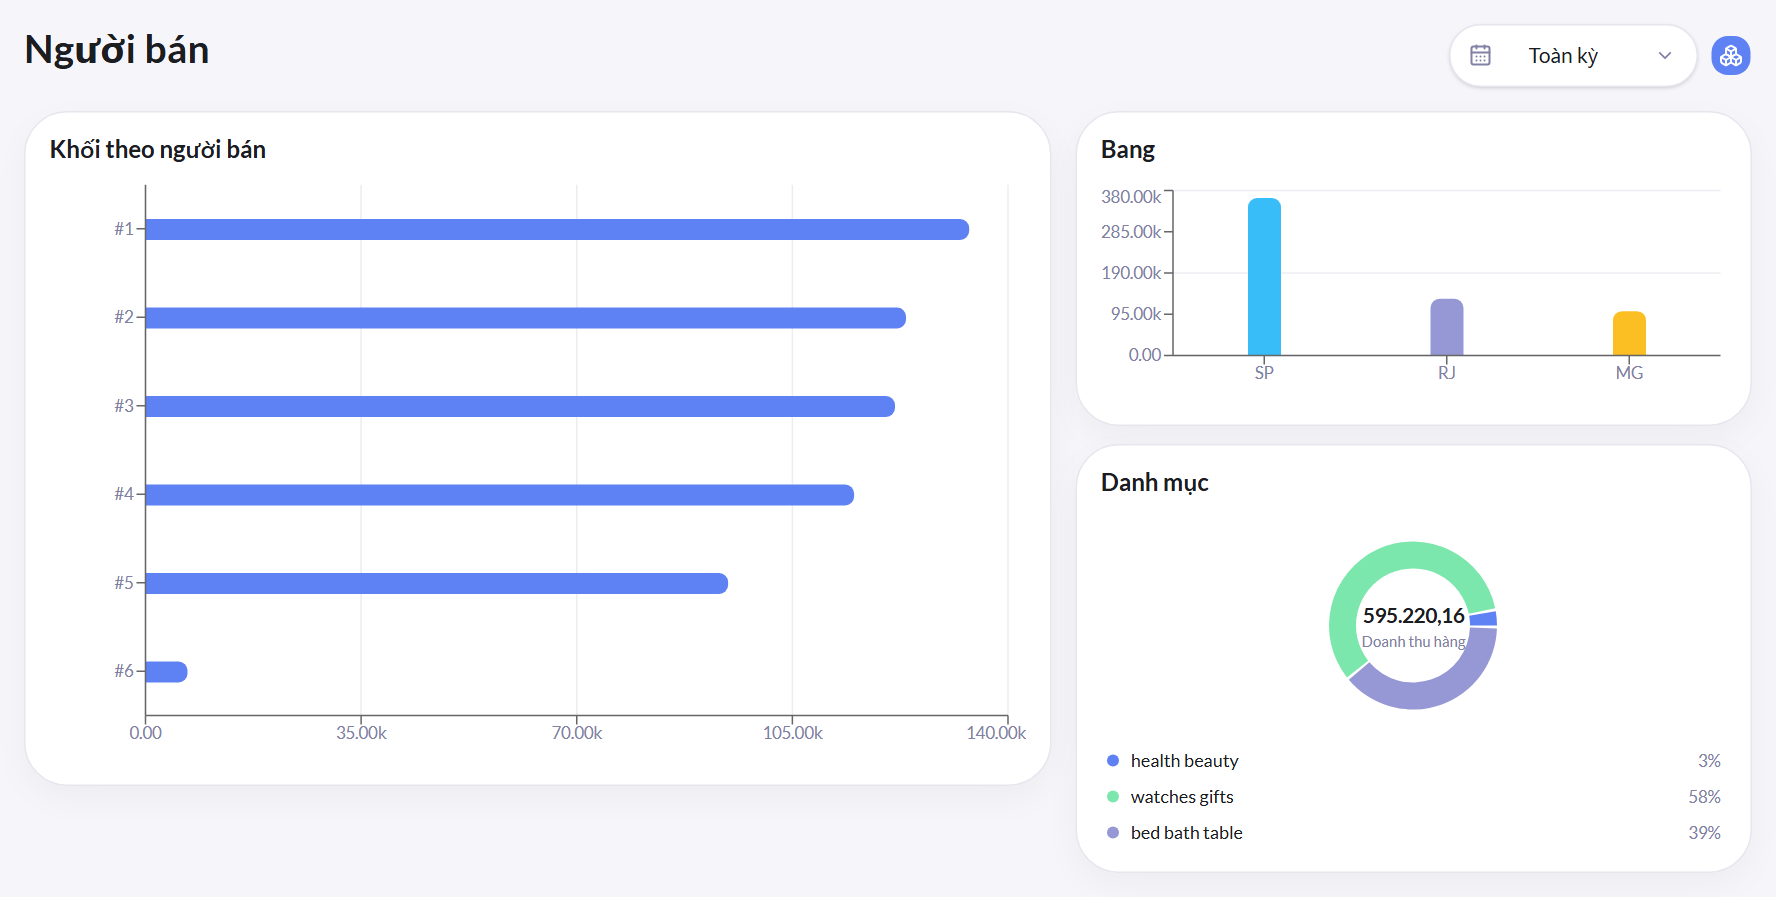
\includegraphics[width=\linewidth,height=0.42\textheight,keepaspectratio]{assets/ui_seller_cube.png}
\caption{Khối người bán $\times$ danh mục $\times$ bang}\label{fig:ui-cube}
\end{figure}

\subsubsection*{Màn Khách hàng}
Biểu đồ đổi giữa bốn thước đo: số khách, số đơn, thanh toán, AOV. Ba chiều drill-down gồm nhóm khách (mua một lần/mua lại), địa lý (bang $\rightarrow$ thành phố) và trạng thái đơn. Chế độ dice chọn nhiều bang và khoảng năm. Bảng chi tiết có thể đổi sang ma trận bang $\times$ năm; ngoài ra có bảng top 3 khách chi tiêu nhiều nhất mỗi bang kèm phân vị toàn quốc. Số khách riêng biệt không cộng xuyên bang hay năm; thành phố drill-down chỉ trả top 15 nên tổng hiển thị có thể nhỏ hơn tổng của bang.

Hình~\ref{fig:ui-customer} là màn Khách hàng theo nhóm mua một lần và mua lại, kèm bảng top 3 khách mỗi bang.

\begin{figure}[H]\centering
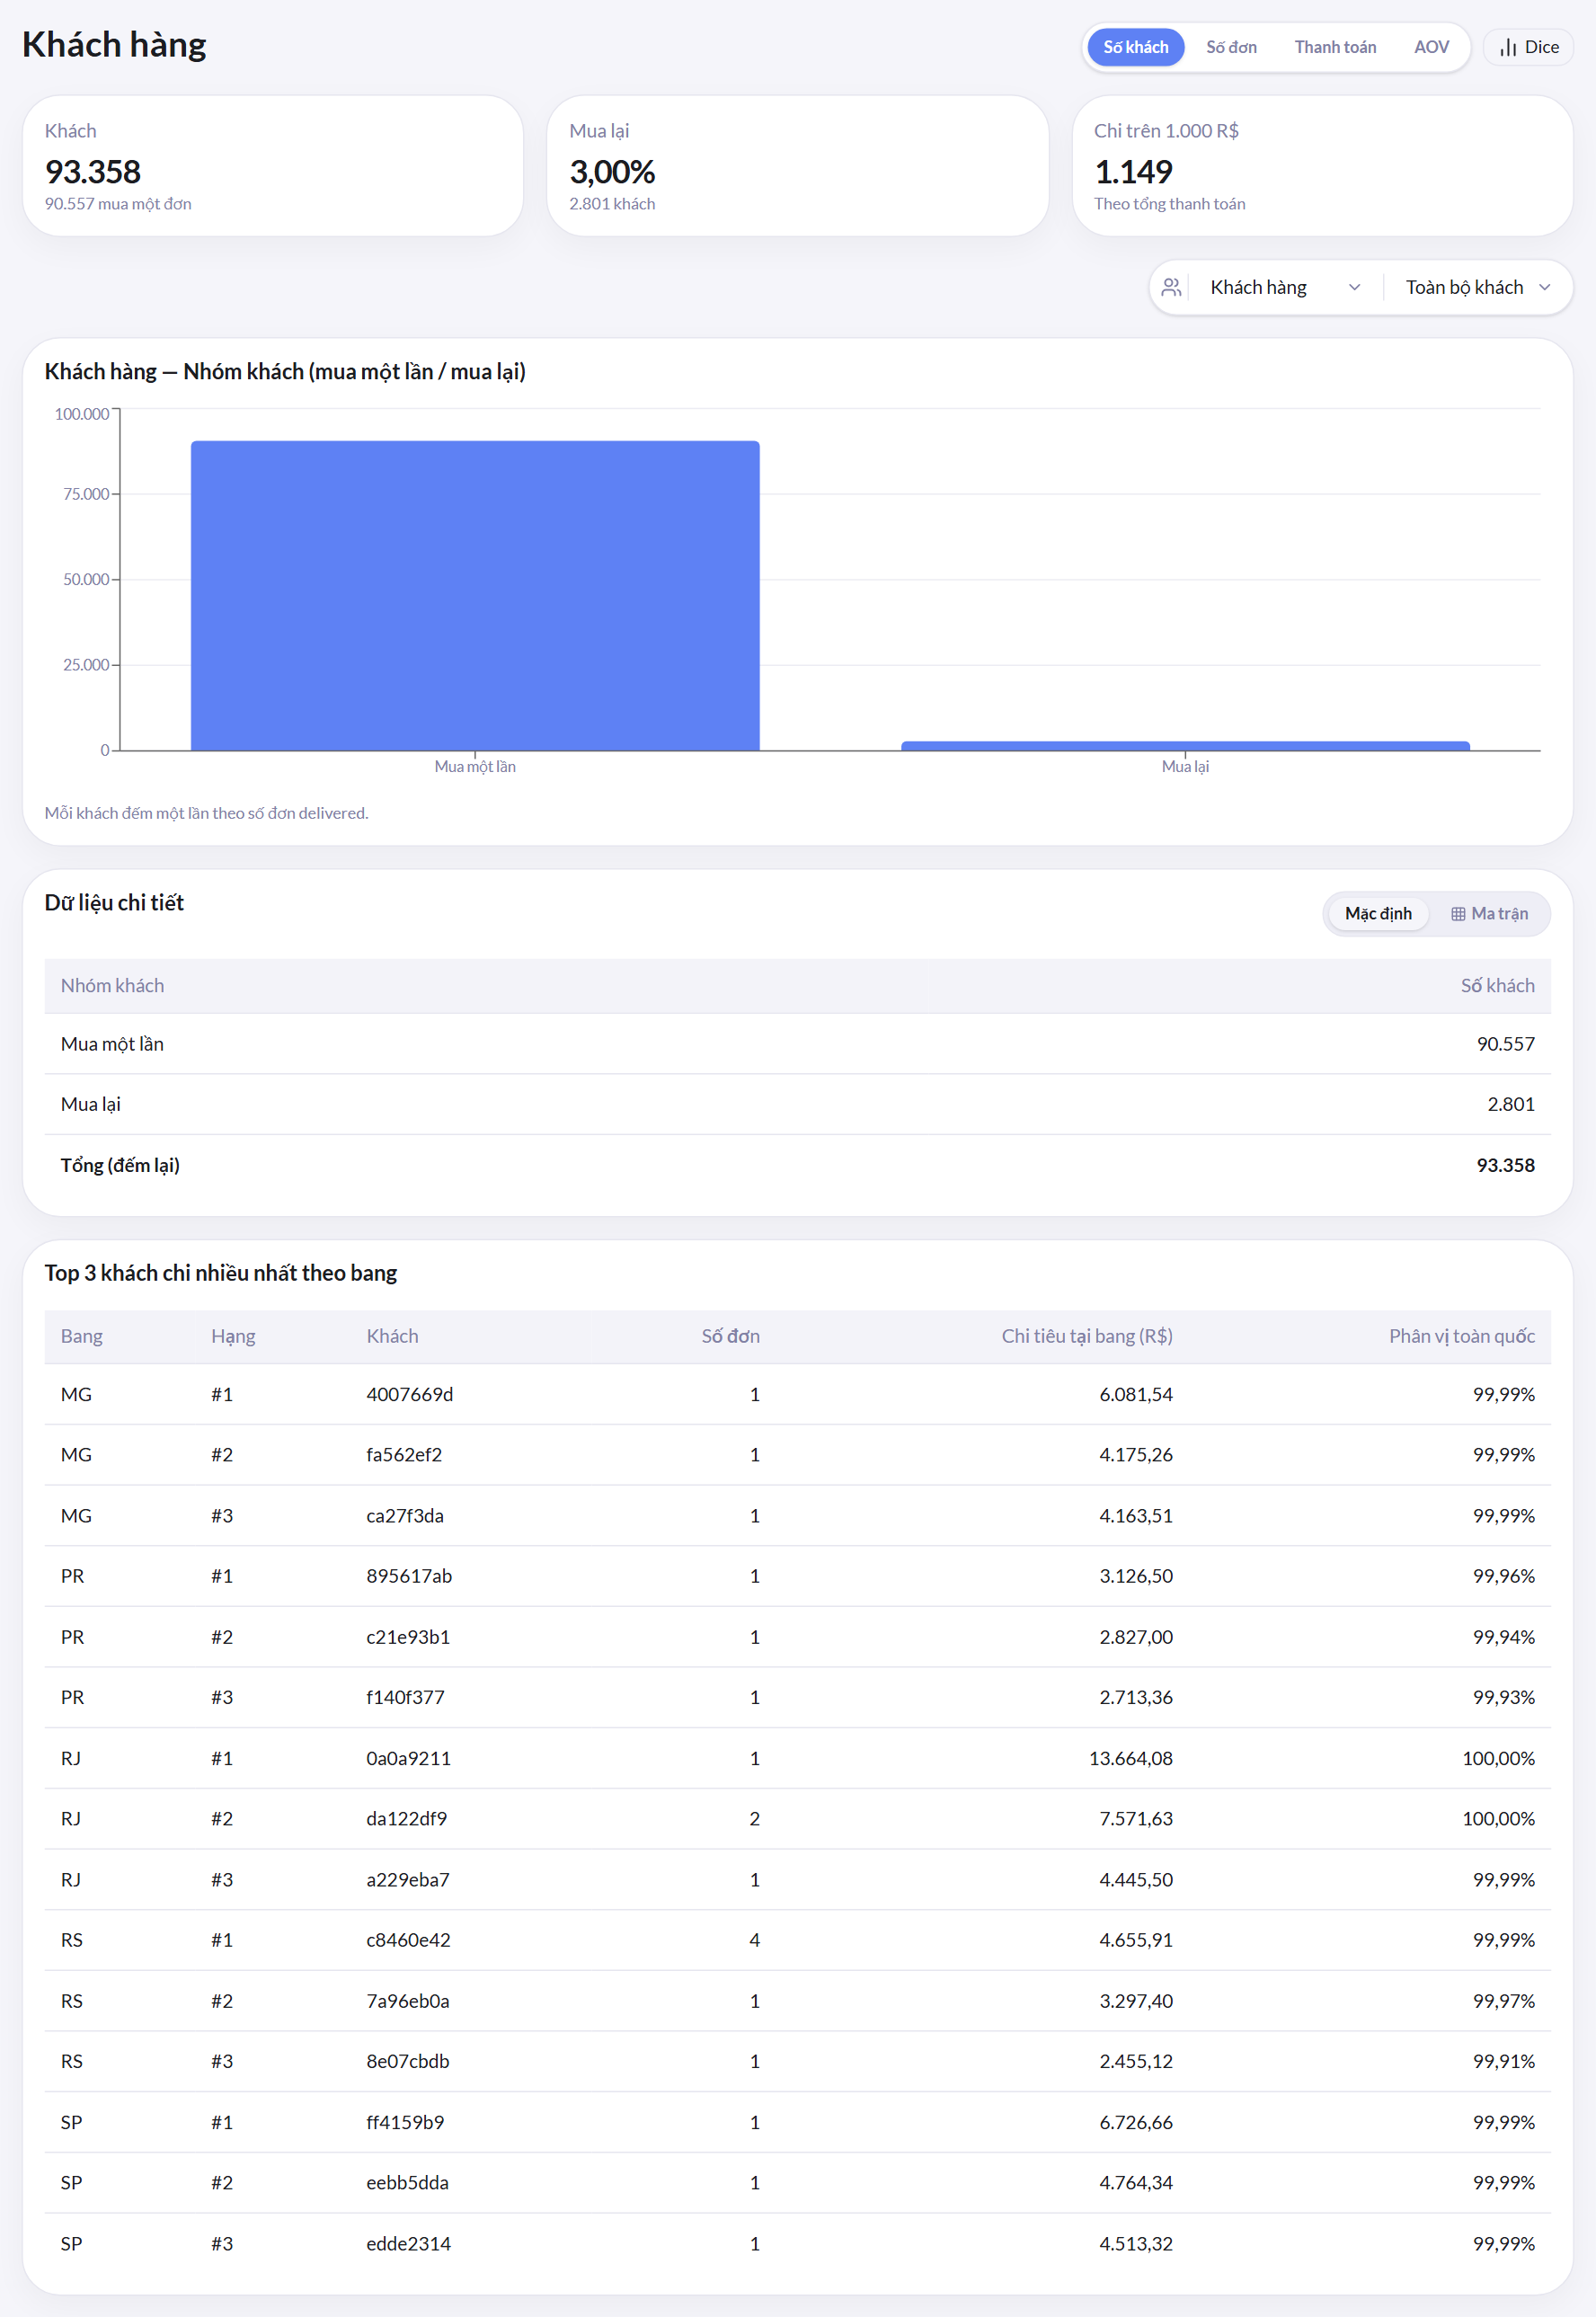
\includegraphics[width=\linewidth,height=0.62\textheight,keepaspectratio]{assets/ui_customer.png}
\caption{Màn Khách hàng}\label{fig:ui-customer}
\end{figure}

\subsection{API và công nghệ hiển thị}
Mỗi màn có nhóm API riêng (\code{/api/sales-time}, \code{/api/olap}, \code{/api/product-geo}, \code{/api/customer-payment}, \code{/api/overview}, \code{/api/dss}). Tên cột SQL lấy từ danh sách cho phép chứ không từ chuỗi truy vấn; giá trị lọc được tham số hóa (riêng năm, quý, tháng ở API Thời gian được ép kiểu số nguyên), tham số sai trả mã 400. Bộ lọc của bốn màn Thời gian, Khu vực, Người bán và Khách hàng được giữ trong URL để chia sẻ trạng thái màn hình, còn màn Người bán dùng lại API Khu vực.

\clearpage\section{Hệ hỗ trợ quyết định: dự báo nhu cầu và lượng nhập}\label{sec:dss}
\subsection{Bài toán và lý do chọn hướng}
Với một phạm vi tùy chọn (toàn kho, một bang hoặc một danh mục), DSS trả lời hai câu hỏi là tháng tới bán được bao nhiêu và nên nhập bao nhiêu.

Hướng ban đầu là phân khúc khách hàng bằng RFM và K-Means. Nhóm đã thử trên dữ liệu thật với kiểm tra theo thời gian (huấn luyện trước, kiểm tra sau) và thấy dữ liệu không đủ thông tin về hành vi quay lại. Cụ thể, 97\% khách (90.557/93.358) chỉ mua một lần nên điểm tần suất gần như hằng số và tỷ lệ mua lại trong 180 ngày chỉ khoảng 3,1\%. K-Means và mô hình có giám sát dùng cùng đặc trưng đều dự đoán việc mua lại chỉ hơn ngẫu nhiên một chút, còn mức đánh giá (review) và việc giao trễ cũng không liên quan đến việc khách mua lại. Ngược lại, nhu cầu theo tháng có thể đo sai số bằng backtest và không cần giả định về hành vi khách, nên DSS chuyển sang dự báo nhu cầu và nhập hàng.

\subsection{Dữ liệu đầu vào}\label{sec:dss-data}
View \code{dw.v_dss_monthly_demand} (\code{sql/dss/01_demand_mart.sql}) tổng hợp đơn delivered theo tháng $\times$ bang $\times$ danh mục với ba cột: số món (\code{units}, số dòng \code{fact_sales}), doanh thu hàng (\code{revenue}) và số đơn. View chỉ đọc kho, không đổi schema và được pipeline tạo lại sau mỗi lần nạp; tổng của nó đối soát khớp với \code{fact_sales} delivered (13.221.498,11 R\$; 110.197 món). Chuỗi lịch sử bắt đầu từ 01/2017 vì đây là tháng đầu của đoạn liên tục. Trước đó, 10/2016 có 313 món nhưng 11/2016 không có đơn nào và 12/2016 chỉ có 1 món. Hai tháng gần như trống này phản ánh khoảng hở của dữ liệu chứ không phải nhu cầu thật; nếu đưa vào, chuỗi sẽ có một cú sụt về 0 rồi bật lên 913 món ở 01/2017, làm Holt học sai xu hướng và làm tăng mẫu số MASE. Hệ thống không nội suy tháng thiếu nên chọn bỏ đoạn này thay vì tự điền số; tháng cuối là tháng gần nhất có số món ít nhất 30\% trung vị các tháng, để một tháng mới nạp dở không bị coi là tháng thật. Với dữ liệu hiện có đó là 08/2018, nên tháng dự báo là 09/2018.

\subsection{Mô hình dự báo và đo sai số}
Chuỗi lịch sử chỉ có khoảng 20 điểm theo tháng nên nhóm chọn các phương pháp đơn giản, ít tham số, thay vì mô hình học máy dễ quá khớp. Bốn cách dự báo trước một tháng được so sánh: naive (lấy tháng trước, dùng làm mốc so sánh), trung bình 3 tháng, Holt có suy giảm xu hướng và kết hợp (trung bình của naive và Holt, là mặc định). Kết hợp được chọn vì naive thường lệch thấp còn Holt lệch cao, nên trung bình bù trừ độ thiên lệch.

Mô hình Holt có suy giảm xu hướng \cite{fpp} dự báo theo công thức
\begin{equation}
\hat y_{t+1}=\ell_t+\phi\, b_t,\qquad 0<\phi<1,
\end{equation}
trong đó $\ell_t$ là mức hiện tại và $b_t$ là xu hướng hiện tại, cả hai được làm mịn theo từng tháng. Nhóm chọn mô hình này vì doanh số 2017--2018 có xu hướng tăng rõ nên cần mô hình có xu hướng, đồng thời hệ số suy giảm $\phi$ làm xu hướng yếu dần theo thời gian, tránh ngoại suy thẳng một đà tăng ngắn hạn. Nói cách khác, dự báo bằng mức hiện tại cộng một phần xu hướng gần nhất; tham số làm mịn và $\phi$ được chọn bằng lưới sao cho sai số dự báo một bước trên lịch sử là nhỏ nhất.

Sai số được đo bằng backtest trượt, tức là với mỗi tháng từ tháng thứ 7 (07/2017) đến 08/2018, mô hình chỉ dùng dữ liệu trước tháng đó, nên sai số đo được mô phỏng đúng tình huống dự báo thật. Sai số được báo cáo bằng hai thước đo, mỗi thước có một lý do riêng:
\begin{align}
\mathrm{WAPE}&=\frac{\sum_t |y_t-\hat y_t|}{\sum_t y_t}\ \text{\cite{kolassa}},\\
\mathrm{MASE}&=\frac{1}{n}\sum_t \frac{|y_t-\hat y_t|}{\mathrm{MAE}^{naive}_{<t}}\ \text{\cite{hyndman}}.
\end{align}
WAPE là tổng sai số tuyệt đối chia tổng lượng bán, tức cho biết ``dự báo lệch bao nhiêu phần trăm so với lượng bán thực''. Thước đo này được chọn thay cho MAPE vì MAPE chia từng tháng riêng nên bị phóng đại ở các tháng bán thấp (ví dụ 2016 hoặc danh mục nhỏ), trong khi WAPE tính trọng số theo quy mô và phù hợp với bài toán tồn kho \cite{kolassa}. MASE chia sai số cho sai số trung bình của dự báo ``tháng trước'' trong dữ liệu đã có tại thời điểm dự báo, nên cho biết mô hình tốt hơn hay kém hơn naive bao nhiêu lần (nhỏ hơn 1 nghĩa là tốt hơn). Thước đo này được thêm vì không phụ thuộc đơn vị, nên so sánh được giữa các bang và danh mục có quy mô rất khác nhau, điều mà WAPE khó làm công bằng; mẫu số chỉ dùng dữ liệu trước tháng dự báo nên không rò rỉ thông tin tương lai \cite{hyndman}.

\subsection{Lượng nhập đề xuất}
Gọi $e_t=y_t-\hat y_t$ là sai số từng tháng backtest (dương nghĩa là cầu vượt dự báo, nguy cơ thiếu hàng). Lượng nhập tháng tới được tính bằng dự báo cộng một khoản đệm an toàn:
\begin{equation}
\text{Lượng nhập}=\max\bigl(\hat y_{\text{tháng tới}}+Q_{p}(e),\,0\bigr),
\end{equation}
với $Q_p$ là phân vị mức $p$ của các sai số $e_t$ (nội suy tuyến tính), $p\in\{85\%,90\%,95\%,99\%\}$ do người dùng chọn, mặc định 90\% \cite{trapero}. Nhóm chọn cách này vì tồn kho an toàn thường được tính bằng công thức dựa trên phân phối chuẩn của sai số, nhưng với 12--14 điểm và sai số lệch (tháng Black Friday), giả định đó không đáng tin; cách phân vị thực nghiệm không cần giả định phân phối và dùng trực tiếp những sai số đã quan sát \cite{trapero}. Ngưỡng 85--99\% là dải mức phục vụ mà bài báo này dùng. Hiểu đơn giản, đệm là mức thiếu hụt mà $p$ phần trăm số tháng quá khứ không vượt quá; đệm có thể âm nếu mô hình thường dự báo cao hơn thực tế.

Vì mẫu nhỏ, mức $p$ danh nghĩa không bảo đảm tỷ lệ không thiếu hàng thực sự. Do đó hệ thống thêm đường đánh đổi đo bằng leave-one-out. Với mỗi tháng, đệm chỉ học từ các tháng khác, lượng nhập của tháng đó là dự báo cộng đệm, rồi đếm tỷ lệ tháng thiếu hàng và mức dư hàng. Cách này được chọn vì mẫu quá ít để chia riêng một tập kiểm tra, trong khi leave-one-out vẫn dùng mọi tháng mà không để tháng nào tự học từ chính nó. Nhờ đó, người ra quyết định thấy được mỗi mức an toàn đánh đổi bằng bao nhiêu hàng dư để giảm bao nhiêu rủi ro thiếu hàng. Công tắc ``bỏ Black Friday khỏi mẫu sai số'' (mặc định bật) loại hai tháng 11--12/2017 vì tháng tới không phải tháng sự kiện.

\subsection{Backend và giao diện}
DSS có ba API là \code{/api/dss/options}, \code{/api/dss/forecast} và \code{/api/dss/accuracy}; phần tính toán nằm trong một mô-đun thuần Python có kiểm thử đơn vị. Màn Quyết định cho chọn phạm vi, thước đo (số món hoặc doanh thu), mức an toàn và cách dự báo. Đầu trang là thẻ kết luận ``Nên nhập khoảng \ldots{} món'', bên dưới là biểu đồ bán thực tế và dự báo, đường đánh đổi theo mức an toàn, sai số theo mức chi tiết và bảng so sánh các cách dự báo.

Hình~\ref{fig:ui-dss} là màn Quyết định cho toàn kho, đo bằng số món, ở mức an toàn 90\%.

\begin{figure}[H]\centering
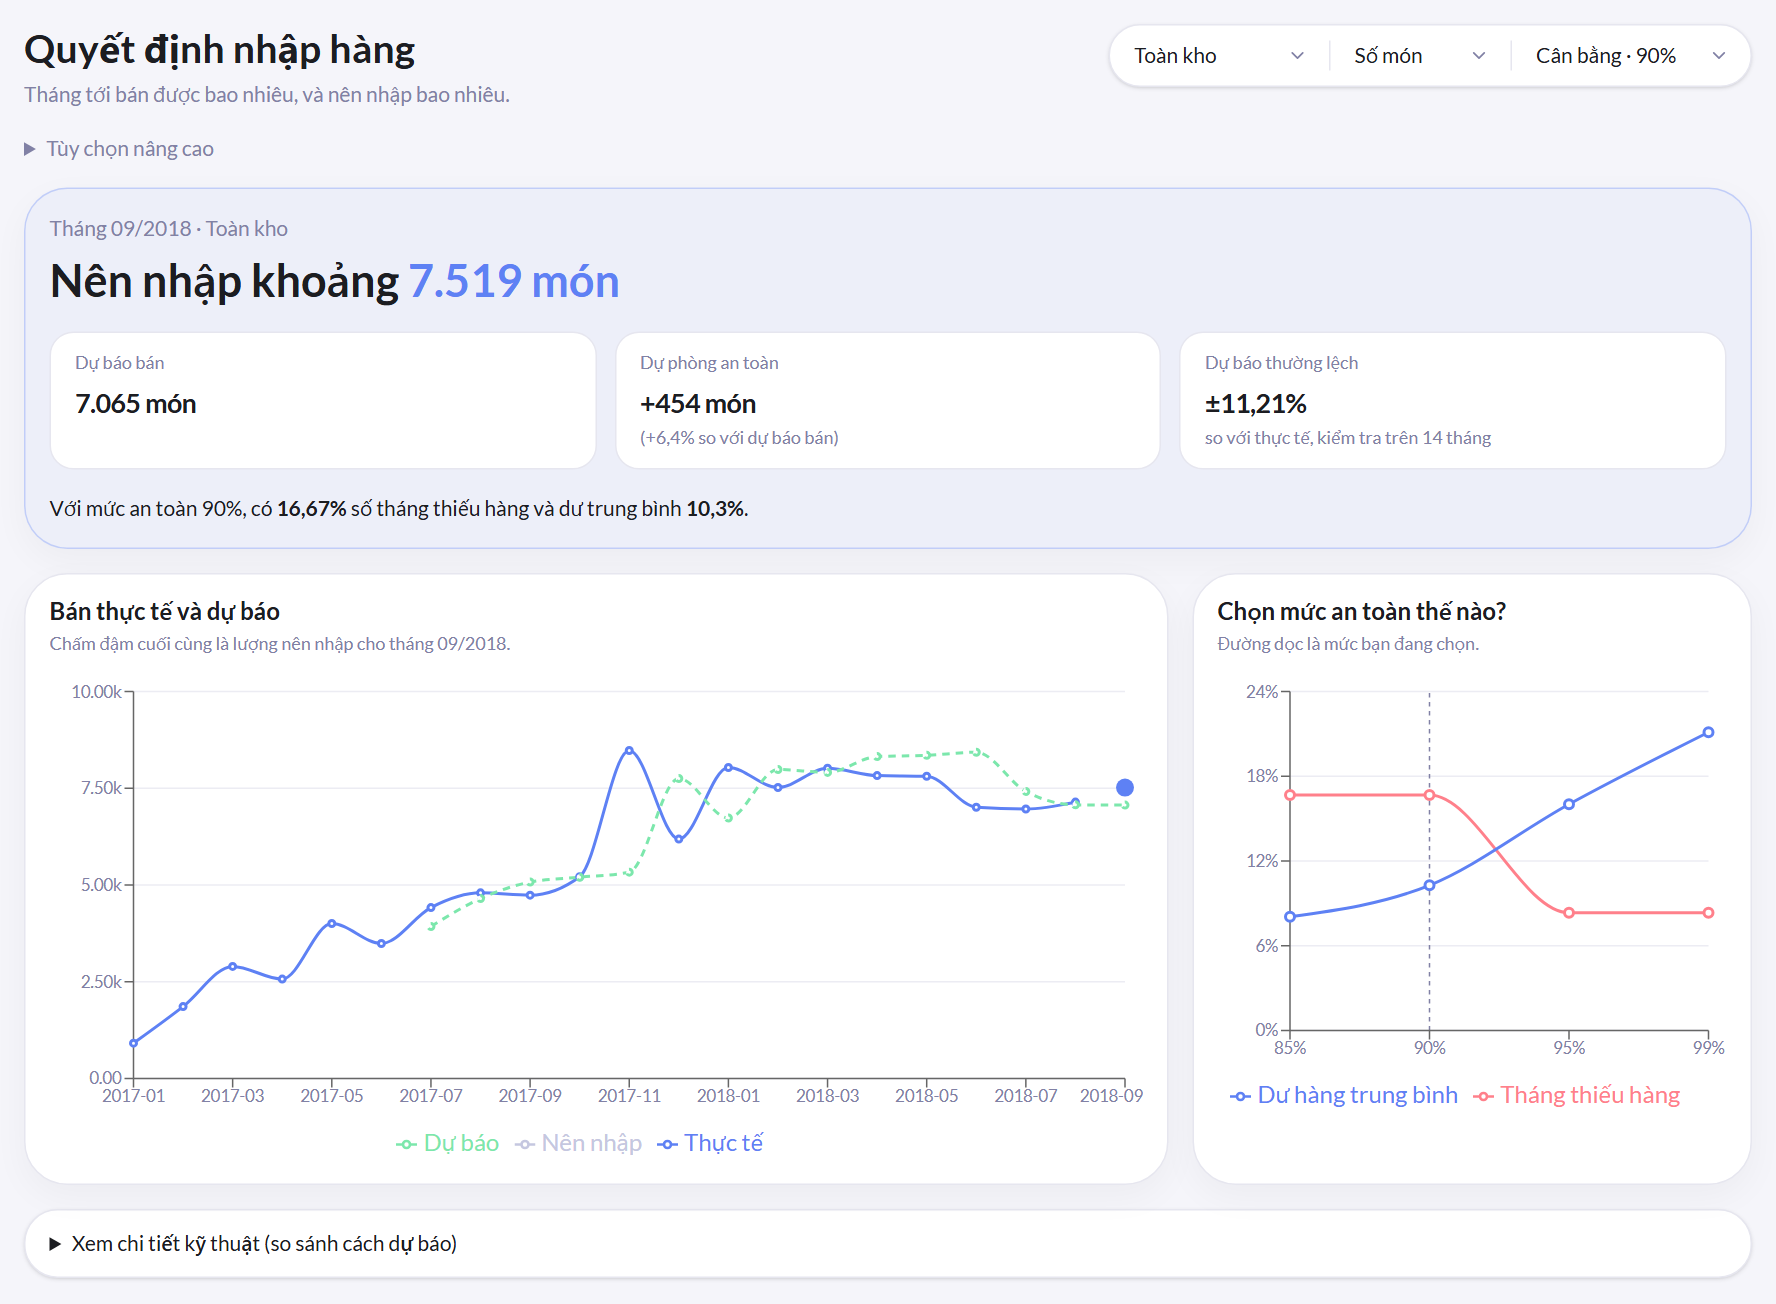
\includegraphics[width=\linewidth,height=0.5\textheight,keepaspectratio]{assets/ui_dss.png}
\caption{Màn Quyết định}\label{fig:ui-dss}
\end{figure}

\subsection{Kết quả}
\begin{table}[H]\centering\small
\begin{tabularx}{\linewidth}{Yr}
\toprule Chỉ số (toàn kho, số món, tháng dự báo 09/2018) & Giá trị\\\midrule
Dự báo bán (mô hình kết hợp) & 7.065 món\\
Đệm ở mức 90\% (bỏ Black Friday, 12 tháng trong mẫu) & +453,64 món (+6,4\%)\\
Lượng nhập đề xuất & 7.518,82 món\\
Tỷ lệ tháng thiếu hàng thực nghiệm ở mức 90\% (leave-one-out) & 16,7\% (2/12 tháng)\\
\bottomrule\end{tabularx}
\caption{Đề xuất nhập hàng toàn kho}
\end{table}

\begin{table}[H]\centering\small
\begin{tabularx}{\linewidth}{Yrrrr}
\toprule Mức tổng hợp & WAPE kết hợp & WAPE tháng trước & MASE kết hợp & MASE tháng trước\\\midrule
Toàn kho & 11,2\% & 12,2\% & 0,88 & 0,97\\
10 bang lớn & 12,9\% & 15,0\% & 1,01 & 1,12\\
15 danh mục lớn & 20,0\% & 20,7\% & 1,23 & 1,27\\
\bottomrule\end{tabularx}
\caption{Sai số backtest theo mức tổng hợp}\label{tab:dssaccuracy}
\end{table}

Mức tổng hợp càng cao càng chính xác. Mô hình kết hợp chỉ hơn mốc ``tháng trước'' một khoảng nhỏ (khi bỏ Black Friday, chênh lệch gần như biến mất, chỉ còn 7,4\% so với 7,5\% ở toàn kho); ở mức bang và danh mục chính mốc naive cũng có MASE trên 1. Có hai lý do. Thứ nhất, giai đoạn kiểm tra biến động mạnh hơn lịch sử. Thứ hai, mỗi chuỗi nhỏ hơn nhiều: theo cách đếm trên CSV với cùng cửa sổ 01/2017--08/2018, trung vị số món mỗi tháng của 10 bang lớn là 231 (từ 110 đến 2.316) và của 15 danh mục lớn là 218,5 (từ 75 đến 557,5), so với khoảng 5.700 ở toàn kho. Chuỗi càng nhỏ thì càng nhiễu, trong khi chỉ có khoảng 20 điểm để học, nên sai số tăng khi xuống mức chi tiết chủ yếu là hệ quả của dữ liệu ít chứ chưa chắc là điểm yếu riêng của mô hình, vì mốc naive cũng chịu cùng mức nhiễu. MASE được dùng để so sánh các mô hình với nhau thay vì so với mốc 1. Tham số số tháng lịch sử tối thiểu ($=6$) do nhóm tự đặt; thay đổi từ 3 đến 10 làm lượng nhập dao động khoảng $\pm 5\%$ quanh 7.500 món (7.214--7.972) và tỷ lệ thiếu hàng thực nghiệm từ 9\% đến 17\%. Vì vậy kết luận nên đọc là ``khoảng 7.500 món'' hơn là một con số chính xác.

\subsection{Hạn chế}
Dữ liệu chỉ có khoảng 20 tháng nên mẫu sai số chỉ 12--14 tháng, làm đệm nhạy với từng tháng bất thường. Tỷ lệ thiếu hàng đo được là 16,7\% (2 trên 12 tháng), cao hơn mức danh nghĩa 10\%, nhưng mỗi tháng thiếu hay không thiếu làm con số đổi khoảng 8,3 điểm phần trăm. Chênh lệch này vì vậy nằm trong mức dao động của mẫu nhỏ và chưa đủ để kết luận cách tính đệm sai; phép thử đổi số tháng lịch sử tối thiểu cũng cho tỷ lệ từ 9\% đến 17\%. Ở mức bang và danh mục, mỗi chuỗi chỉ có vài trăm món mỗi tháng nên sai số lớn hơn toàn kho. DSS chỉ dự báo trước một tháng, chưa có khoảng dự báo dạng băng trên biểu đồ và chưa xét tồn kho hiện có hay thời gian giao hàng của nhà cung cấp.

\clearpage\section{Kết quả kiểm chứng và thảo luận}\label{sec:results}
\subsection{Phương pháp kiểm chứng}
Kết quả được kiểm chứng ở ba lớp: (1) tính lại các chỉ số trực tiếp từ CSV độc lập với kho, tiền được đổi sang cent nguyên trước khi cộng để tránh sai số nhị phân; (2) chạy đầy đủ pipeline nạp trên PostgreSQL 16 cùng bộ nghiệm thu F1--F7 và các script đối soát; (3) kiểm thử mã (unit test và gọi API). Các số trong chương này đã được tính lại trên kho vừa nạp và khớp với kết quả tính từ CSV. Ngoài thời gian chạy pipeline, báo cáo không đo độ trễ API hay hiệu năng truy vấn.

\begin{table}[H]\centering\small\renewcommand{\arraystretch}{1.15}
\begin{tabularx}{\linewidth}{>{\raggedright\arraybackslash}p{0.5\linewidth}Y}
\toprule Hạng mục & Kết quả\\\midrule
Pipeline nạp đầy đủ (PostgreSQL 16) và nghiệm thu F1--F7 & Hoàn tất trong khoảng 48 giây, đạt.\\
Giả lập lỗi ở bước nghiệm thu & Pipeline dừng, toàn bộ lần nạp bị rollback, kho cũ nguyên vẹn.\\
Đối soát view DSS với \code{fact_sales} delivered & Khớp ở 13.221.498,11 R\$ và 110.197 món.\\
Đối soát OLAP Khu vực/Người bán (nền, roll-up, drill-down, cộng bang, cộng thành phố, dice, top 3 theo bang) & 4/4 đạt.\\
Gọi API bằng Flask test client (Tổng quan, Thời gian, Khu vực/Người bán, Khách hàng, Quyết định) & 31/31 URL hợp lệ trả mã 200; 3 URL tham số sai trả mã 400.\\
Unit test (tính toán DSS, tăng trưởng cùng kỳ, ngưỡng tháng thưa và số tháng tối thiểu của MoM, QoQ, YoY) & 19/19 đạt.\\
\bottomrule\end{tabularx}
\caption{Kết quả kiểm thử}
\end{table}

\subsection{KPI của kho}
\begingroup\small\renewcommand{\arraystretch}{1.15}
\begin{longtable}{p{0.70\linewidth}r}
\caption{KPI của kho}\label{tab:kpi}\\
\toprule Chỉ số & Giá trị\\\midrule\endfirsthead
\toprule Chỉ số & Giá trị\\\midrule\endhead
\bottomrule\endfoot
Đơn hàng (mọi trạng thái) & 99.441 \\
Dòng sản phẩm (mọi trạng thái) & 112.650 \\
Đơn delivered & 96.478 \\
Dòng sản phẩm delivered & 110.197 \\
Khách có đơn delivered & 93.358 \\
Đơn delivered có thanh toán & 96.477 \\
Đơn delivered thiếu thanh toán & 1 \\
Doanh thu hàng delivered (R\$) & 13.221.498,11 \\
Cước delivered (R\$) & 2.198.275,64 \\
Thanh toán delivered (R\$) & 15.422.461,77 \\
AOV trên đơn có thanh toán (R\$) & 159,86 \\
Khách mua một lần & 90.557 \\
Khách mua lại & 2.801 \\
Tỷ lệ khách mua lại (\%) & 3,00 \\
\end{longtable}\endgroup

Doanh thu hàng cộng cước là 15.419.773,75 R\$, thấp hơn tổng thanh toán 2.688,02 R\$. Hai nhóm thước đo ở grain khác nhau và dữ liệu không có quy tắc đối soát kế toán, nên báo cáo không suy đoán nguyên nhân chênh lệch. Một đơn delivered không có dòng payment được giữ NULL, vì vậy AOV chia cho 96.477 đơn có dữ liệu. Tỷ lệ mua lại 3\% chỉ mô tả cửa sổ quan sát trong dataset, không có nghĩa 97\% khách còn lại đã rời bỏ.

\subsection{Thời gian và danh mục}
\begin{table}[H]\centering\small
\begin{tabularx}{\linewidth}{rYrr}
\toprule Năm mua & Phạm vi dữ liệu delivered & Đơn delivered & Doanh thu hàng (R\$)\\\midrule
2016 & Từ 15/09, thiếu tháng 11 & 267 & 40.470,98\\
2017 & Đủ 12 tháng & 43.428 & 5.962.902,01\\
2018 & Đến 29/08 (tháng 1--8) & 52.783 & 7.218.125,12\\
\bottomrule\end{tabularx}
\caption{Tổng hợp theo năm mua}
\end{table}
Ba năm không cùng số tháng nên tăng trưởng được so theo cùng kỳ. Cụ thể, 2018 (tháng 1--8) so với tháng 1--8 của 2017 tăng +141,13\% (2.993.456 $\rightarrow$ 7.218.125 R\$); quý 3/2018 (chỉ có tháng 7--8) so với tháng 4--5 của quý 2 giảm 12,53\%. YoY của 2017 so với 2016 để trống vì chỉ có một cặp tháng hợp lệ (quy tắc ở chương~\ref{sec:olap}), thay vì +4.796\% khi ghép cả các tháng gần như trống; 2016 chỉ là giai đoạn khởi động với vài đơn mỗi tháng nên không mang ý nghĩa kinh doanh. Chuỗi DSS cũng bắt đầu từ 2017 vì khoảng hở 11--12/2016 (mục~\ref{sec:dss-data}).

\begin{figure}[H]\centering
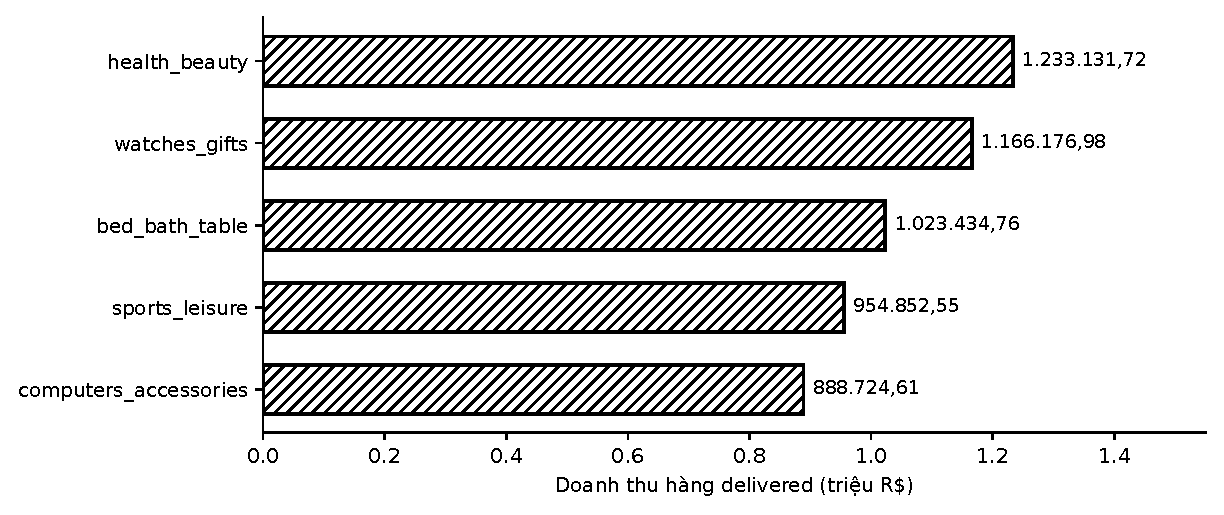
\includegraphics[width=\linewidth]{assets/fig_top_categories.pdf}
\caption{Top 5 danh mục theo doanh thu}
\label{fig:categories}
\end{figure}
Danh mục \code{health_beauty} đứng đầu với 1.233.131,72 R\$, tiếp theo là \code{watches_gifts} và \code{bed_bath_table}. Doanh thu hàng không phải lợi nhuận, nên đây là cơ sở chọn danh mục để phân tích sâu chứ chưa phải căn cứ về hiệu quả kinh doanh.

\subsection{Chất lượng nguồn}
\begin{table}[H]\centering\small
\begin{tabularx}{\linewidth}{YrY}
\toprule Kiểm tra / quan sát & Kết quả & Cách hiểu\\\midrule
Trùng khóa hoặc khóa rỗng ở 7 nguồn nạp & 0 & Theo khóa mà staging khai báo.\\
Orphan ở 5 liên kết nguồn & 0 & Orders--customers; items--orders/products/sellers; payments--orders.\\
Giá, cước, payment âm & 0 & Quan sát từ CSV.\\
Sản phẩm thiếu danh mục & 610 & NULLIF giữ thiếu, không tự gán.\\
Sản phẩm có danh mục chưa có bản dịch & 13 & Hai danh mục \code{pc_gamer} và \code{portateis_cozinha_e_preparadores_de_alimentos}; LEFT JOIN giữ sản phẩm.\\
Đơn thiếu ngày duyệt & 160 & \code{approved_date_key} cho phép NULL.\\
Đơn không có dòng hàng (mọi trạng thái) & 775 & Cardinality order--item là 0..N.\\
\bottomrule\end{tabularx}
\caption{Chất lượng dữ liệu nguồn}
\end{table}

\subsection{Giới hạn của kết luận}
Giao diện được kiểm tra ở mức biên dịch và lớp API; chưa có kiểm thử tự động trên trình duyệt, màn hình hẹp hay nhiều trình duyệt. Chưa có đo hiệu năng. Kết quả DSS dựa trên 14 tháng backtest, và ở mức bang, danh mục mỗi chuỗi chỉ có vài trăm món mỗi tháng, nên chỉ có giá trị ước lượng thô (chương~\ref{sec:dss}).

\clearpage\section{Kết luận, hạn chế và hướng phát triển}
\subsection{Kết quả đạt được}
Dự án xây dựng một kho dữ liệu đa chiều gồm staging, bốn dimension và hai fact (grain dòng hàng và grain đơn), nạp bằng pipeline COPY và SQL, có bộ nghiệm thu F1--F7 và chạy trong một giao dịch (chỉ commit khi hợp lệ). Việc tách grain thanh toán khỏi dòng hàng tránh nhân bản tiền, và định danh khách duy nhất cho phép phân tích mua lại. Trên kho là một ứng dụng web có API Flask và sáu màn hình: Tổng quan, Thời gian, Khu vực, Người bán, Khách hàng và Quyết định, hỗ trợ các thao tác drill-down, roll-up, slice, dice và pivot. Tăng trưởng theo năm và quý được tính cùng kỳ để không bị sai lệch bởi dữ liệu thiếu tháng.

Thành phần DSS dự báo nhu cầu theo tháng và đề xuất lượng nhập với mức an toàn do người dùng chọn. Với tháng 09/2018, hệ thống dự báo 7.065 món và đề xuất nhập khoảng 7.519 món ở mức 90\%, với sai số WAPE 11,2\% ở mức toàn kho. Phân khúc khách hàng đã được thử và bị loại do dữ liệu không chứa tín hiệu về việc khách quay lại.

\subsection{Hạn chế}
\begin{itemize}[leftmargin=*]
\item Dữ liệu chỉ phủ khoảng 24 tháng, năm 2016 rất thưa; mẫu backtest DSS chỉ 12--14 tháng nên đệm nhập hàng là ước lượng thô. Tỷ lệ thiếu hàng đo được (16,7\%) cao hơn mức danh nghĩa 10\%, nhưng một tháng đã làm con số đổi khoảng 8,3 điểm phần trăm; sai số ở mức bang và danh mục cũng lớn hơn toàn kho vì mỗi chuỗi chỉ có vài trăm món mỗi tháng. Các kết quả chưa tốt này nên được đọc là hệ quả của dữ liệu ít, và cần chuỗi dài hơn mới kết luận được về mô hình.
\item DSS chỉ dự báo trước một tháng, chưa có khoảng dự báo, chưa xét tồn kho hiện có, giá vốn hay khuyến mãi.
\item Kho không có SCD, loại thanh toán, review và thời gian giao hàng; chưa nạp tăng dần nên mỗi lần nạp lại phải xây lại toàn bộ.
\item Chưa đo hiệu năng và chưa kiểm thử giao diện trên nhiều trình duyệt hoặc màn hình hẹp.
\end{itemize}

\subsection{Hướng phát triển}
Bổ sung dữ liệu nhiều tháng hơn để kiểm chứng đệm nhập hàng và sai số ở mức bang, danh mục; nạp thêm review, thời gian giao hàng và loại thanh toán để mở rộng chiều phân tích; nạp tăng dần và logging; dự báo nhiều tháng kèm khoảng dự báo; bổ sung giá vốn và dữ liệu khuyến mãi để có thể đánh giá kịch bản định giá.

\clearpage\phantomsection\addcontentsline{toc}{section}{Tài liệu tham khảo}
\begin{thebibliography}{9}
\bibitem{kimball} R. Kimball, M. Ross, \textit{The Data Warehouse Toolkit}, 3rd ed., Wiley, 2013.
\bibitem{olist} Olist, \textit{Brazilian E-Commerce Public Dataset by Olist}, Kaggle.
\bibitem{fpp} R. J. Hyndman, G. Athanasopoulos, \textit{Forecasting: Principles and Practice}, 3rd ed., OTexts, 2021 (chương 8, mục 8.2 ``Methods with trend'', phần Damped trend methods). \url{https://otexts.com/fpp3/}
\bibitem{kolassa} S. Kolassa, W. Schütz, ``Advantages of the MAD/Mean ratio over the MAPE'', \textit{Foresight} 6, 2007, 40--43.
\bibitem{hyndman} R. J. Hyndman, A. B. Koehler, ``Another look at measures of forecast accuracy'', \textit{International Journal of Forecasting} 22(4), 2006, 679--688.
\bibitem{trapero} J. R. Trapero, M. Cardós, N. Kourentzes, ``Empirical safety stock estimation based on kernel and GARCH models'', \textit{Omega} 84, 2019, 199--211.
\end{thebibliography}

\end{document}
